
\special{papersize=8.5in,11in}
\documentclass[titlepage,12pt] {article}  
\usepackage{setspace}
\topmargin =-1.5cm \evensidemargin = -0.02in
\oddsidemargin=-0.02in \textwidth=16.5cm \textheight=24cm
\usepackage{fullpage}

%uncomment this to put figures at end
%\usepackage[nomarkers, fighead]{endfloat}

\usepackage{color}
\usepackage{array}
\newcommand{\N}[2]{{\mbox{$\cal N\!\,$$\left({#1},{#2}\right)$}}}
\newcommand{\tcr}{\textcolor{black}}
\def\baselinestretch{1}
\usepackage{natbib}
 \usepackage{graphics}
\usepackage{graphicx}
 \usepackage{epsfig}
\usepackage{amssymb}
\usepackage{amsmath}
\usepackage{alltt}
\usepackage{multirow}
\usepackage{hyperref}
\usepackage{physics}
\usepackage{xcolor}
\newcommand{\gr}{\textbf{(get ref)}}
\newcommand{\gf}{\textbf{(get fig)}}
\usepackage{caption}
\usepackage{subcaption}
\newcommand{\jb}[1]{\textcolor{red}{{#1}}}  
\newcommand{\jbnote}[1]{\textcolor{blue}{{#1}}}  
%\newcommand{\jb}{} % to remove color of jb 
%\newcommand{\jbnote}{} % to remove color of jbnote
\newcommand{\bi}{\begin{itemize}}
\newcommand{\ei}{\end{itemize}}

\newcolumntype{L}[1]{>{\raggedright\let\newline\\\arraybackslash\hspace{0pt}}m{#1}}

\newcommand{\rh}{\textcolor{magenta}{\textbf{(Russ, help)}}}
\newcommand{\ph}{\textcolor{magenta}{\textbf{(Patrick, help)}}}
\newcommand{\jm}[1]{\textcolor{orange}{{#1}}}  
\usepackage{chngcntr}

\newcommand{\beginsupplement}{%
        \setcounter{table}{0}
        \renewcommand{\thetable}{S\arabic{table}}%
        \setcounter{figure}{0}
        \renewcommand{\thefigure}{S\arabic{figure}}%
     }

\begin{document}


\begin{titlepage}
\begin{center}
{\large\textbf{The response time paradox in functional magnetic resonance imaging analyses
}}\\
{Jeanette A. Mumford$^1$, Patrick Bissett$^1$, Henry Jones$^2$, Sunjae Shim$^1$, Jaime Rios$^1$, Russell A Poldrack$^1$\\
  \small{1} Department of Psychology, Stanford University }
\end{center}


\textbf{(Target journal = elife)}

\vspace{2.8in}
\begin{singlespace}
  \hspace{0.1in}\newline
\textbf{Correspondence}\newline 
Jeanette A Mumford, Ph.D. \newline 
jeanette.mumford@gmail.com \newline
\end{singlespace}

\newpage
\noindent {\em Abstract:}
%150-200 words

Testing github.  
The signal measured using functional MRI (fMRI) is a proxy for an unobservable neuronal signal. Changes in intensity and duration of neuronal activity can yield identical changes in fMRI signals, but the actual duration of the neuronal response is generally unknown, which means that differences in response times may lead to spurious differences in fMRI signals that do not reflect differences in the intensity of neuronal activity.  This raises a paradox, given that differences in response times are present for almost every contrast of interest in task fMRI: The difference of interest in one variable of interest (RT) reflects a potential confound for another variable of interest (fMRI).  Although this problem was first raised more than a decade ago, analysis practices have remained largely unchanged.  Here we propose a new modeling strategy that separates condition differences from response time differences with the ability to adapt to either constant or varying durations of neuronal response.  This model controls type I errors, while retaining the same level of power as the (generally unknown) correct model.  We further demonstrate that the failure to address response time in the modeling of data from individual participants leads to a previously unknown response time confound in group comparisons and associations, even when average RT differences are zero.  In addition to offering time series analysis solutions, we discuss limitation and fixes when the time series analysis decisions are out of the hands of the researcher, as when using activation map estimates from shared datasets.


\vspace{.1in}
\noindent {\small{\em Keywords:} fMRI, response time, modeling, group confound}


\end{titlepage}

\section*{Introduction}

The goal of task-based functional magnetic resonance imaging (fMRI) studies is to infer the involvement of particular brain regions or networks in specific cognitive functions.  Using the subtraction logic first developed by \citet{donders1969} for the analysis of response times (RTs), comparisons are made between different task conditions that are thought to differ with regard to the involvement of some specific cognitive function.  For example, in the well known Stroop task, stimuli are presented in which the color and text of the word are either congruent (e.g.\ ``blue" presented in blue) or incongruent (e.g.\ ``blue" presented in red).  Individuals are consistently slower at naming the color of the stimulus when the written word is incongruent compared to congruent, and this difference in response times is interpreted as indexing the engagement of an additional cognitive process in the incongruent condition, such as conflict detection or resolution \citep{botvinick2001}. Similarly, greater activation in regions such as the dorsal medial frontal cortex (dMFC) in fMRI studies of the Stroop task have been interpreted as reflecting a specific role for those regions in this additional cognitive process (REFS \ph).  

There is, however, a fundamental confound in the interpretation of task fMRI signals when response times differ between the conditions being compared. Because of the slow nature of the blood oxygen-level dependent (BOLD) response that is measured in most fMRI studies, it is nearly impossible to distinguish the degree to which a difference in evoked BOLD response reflects either an increase in the amplitude of neuronal response in a region versus a difference in the duration of that response (Figure \ref{fig:neuron_bold}).  This indeterminacy has been known since the early days of fmri \citep{savoy1995, fslbook2001}, and its impact on the interpretation of task fMRI signals was the focus of a set of studies published more than a decade ago  \citep{grinband_detection_2008,  carp_conditional_2010, grinband_dorsal_2011, weissman_congruency_2013}.  Its central importance for task fMRI research arises from the fact that the large majority of task fMRI manipulations lead to longer response times in the more vs. less complex task condition, would be expected given that the logic of subtraction derives directly from the design of response time experiments.

\begin{figure}[h!]
  \centering
   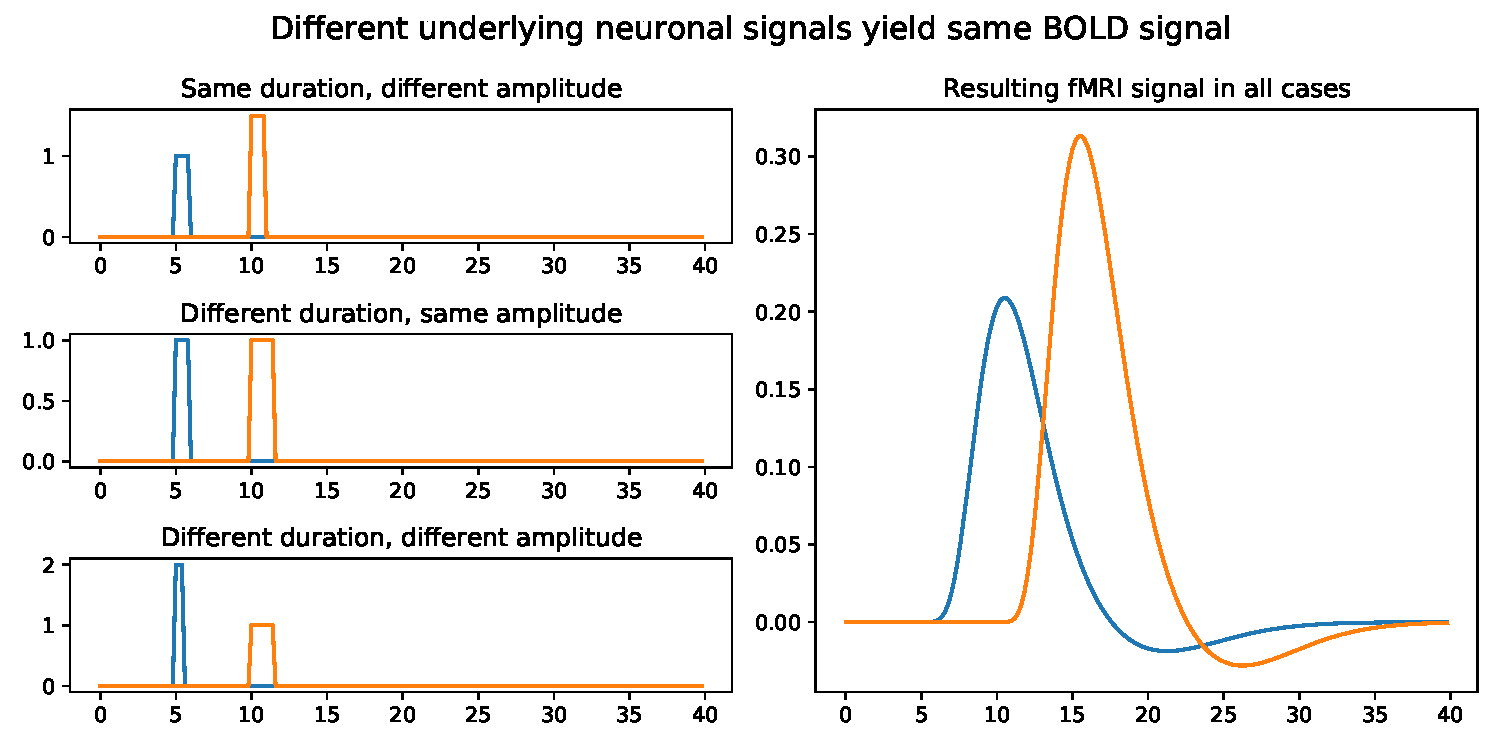
\includegraphics[width=4in]{Figures/neuron_same_bold.pdf}
   \caption{Illustration of how amplitude and duration of neuronal signal interact to yield similar BOLD responses.  The left hand column shows 3 different examples of neuronal signals that evoke the same BOLD response shown in the right hand panel.   }
  \label{fig:neuron_bold}
 \end{figure}

\citet{grinband_detection_2008} showed that it is possible to statistically control for the effects of response times, so that the resulting inferences can be interpreted more specifically with regard to underlying cognitive processes without the confound of differences in response times.  In the context of the Stroop task, \citet{grinband_dorsal_2011} showed that the difference in dMFC activation between slow and fast congruent trials was similar to the difference between all congruent and incongruent trials.  This finding undercuts the interpretation of dMFC activation, as it is not clear whether it reflects the putative Stroop effect or simply reflects longer response times on incongruent trials.  A different approach to statistically control for RT in the Stroop task was used in \citet{carp_conditional_2010} and illustrated that the network of activation differences between incongruent and congruent activation, beyond and including the dMFC, is largely confounded by the RT effect.  This set of brain regions is part of a now well-established network whose activity varies with RTs in a way that is relatively independent of the particular task being performed.  \citet{yarkoni_bold_2009} examined the relationship between RT and fMRI signal across different tasks, and found that there was a network of brain regions whose activity was correlated with RT across all of the tasks. Together these findings raise significant concern that condition differences found in fMRI literature may be reflective of an RT difference between the conditions rather than qualitative differences in process engagement between conditions.  


Accounting for RT-based time on task effects may question the current interpretations of brain involvement with different tasks.  Even though the compelling work of \citet{grinband_dorsal_2011} opened the discussion to further question and understand the underlying theoretical model of this task \citep{yeung_errors_2011, brown_medial_2011, alexander_medial_2011, brown_medial_2011}, there was not a strong conclusion and the impact on how the Stroop task is analyzed and interpreted in fMRI research is largely unaffected. Despite the knowledge of this potential confound, very few published fMRI studies have addressed RTs in their analyses.  For example, of the 22 papers published resulting from a PubMed search for ``stroop task fmri 2021'' that focused on condition differences in the task, only 4 addressed RT in their analyses and interpretation of their results. Thus, interpretations of a substantial proportion of the task fMRI literature may be challenged by the failure to address this challenge, and the use of modeling approaches to address this confound are likely to improve the interpretability of task fMRI results.
%Analyzing the effects in parallel, RT-based effects and condition effects adjusted for RT, will improve the understanding of the brain.

Prior work studying RT as a confound in fMRI models has focused on RT adjustment in the time series model, or between-trial differences in RT, where the aim is to avoid false positive detections in group averages of condition differences in fMRI activation when those conditions have different RTs.  A second problem, introduced in the present work, is that correlations with fMRI contrasts of condition differences can be confounded by RT at the group level regardless of whether RT differs between conditions; this highlights the importance of RTs as a confound in \emph{group} analyses.  These between-subject RT effects may be as large or larger than the size of effects that are typically of interest, e.g. correlations with different phenotypes.  Given the substantial interest in the brain-behavior relationships in the fMRI literature, this is a confound of major importance to the field.


In the present paper we aim to bring renewed attention to the confound of response times in task fMRI studies.  First, we present a set of simulations that demonstrate the impact of RT differences on the interpretation of condition differences in fMRI signals.  These simulations show that the strategy developed by \citet{grinband_detection_2008} relies upon problematic assumptions regarding the relationship between response times and BOLD responses across the brain, whereas a more flexible model of RT can remove their confounding effects without the bias arising from those limiting assumptions.  Importantly, this new model is shown to have adequate statistical power.  Second, we demonstrate that RT differences between subjects can `leak' into group analyses, resulting in potential confounding of individual difference analyses. We also replicate and extend the findings of \citet{yarkoni_bold_2009} by demonstrating that the widespread associatoin between RT and fMRI activation is consistent over a set of 7 fMRI tasks. We propose that these results suggest the need for more common usage of appropriate response time modeling strategies in fMRI studies.  It especially important to consider the impact of the chosen time series model and whether or not it adjusted for RTs when using fMRI contrast estimates provided in databases for large scale neuroimaging studies.  Limitations and some solutions to remove the impact of RTs in this situation are discussed along with other practical modeling choices.

\section*{Results}

\subsubsection*{Simulations}

The statistical models used for fMRI data generally involve the convolution of a vector representing trial or stimulus onsets with a canonical hemodynamic response function (as shown in Figure \ref{fig:neuron_bold})  to create regressors for use in linear modeling \citep{PoldrackMumfordNichols2009}.  The trials can be represented either as delta functions or as boxcar functions with some duration; when a boxcar is used, it is common to set the duration of the boxcar to a constant value such as the duration of the stimulus, or to some default value (such as 0.1 second).  In Figure \ref{fig:models} this model is referred to as ``Constant duration, no RT'' (hereafter as ConstDurNoRT).  Because of the indeterminacy described above, the specific constant value used for stimulus duration will not generally impact the statistical inferences derived from the model, as it will simply scale the values of the parameter estimates along with their variances (assuming the trial durations are relatively short).   This standard approach does not include any information about response times; thus, if two conditions differ in their RTs when the true activation magnitude does not differ, the condition with the longer RTs will have higher estimated activation.  

\begin{figure}
  \centering
   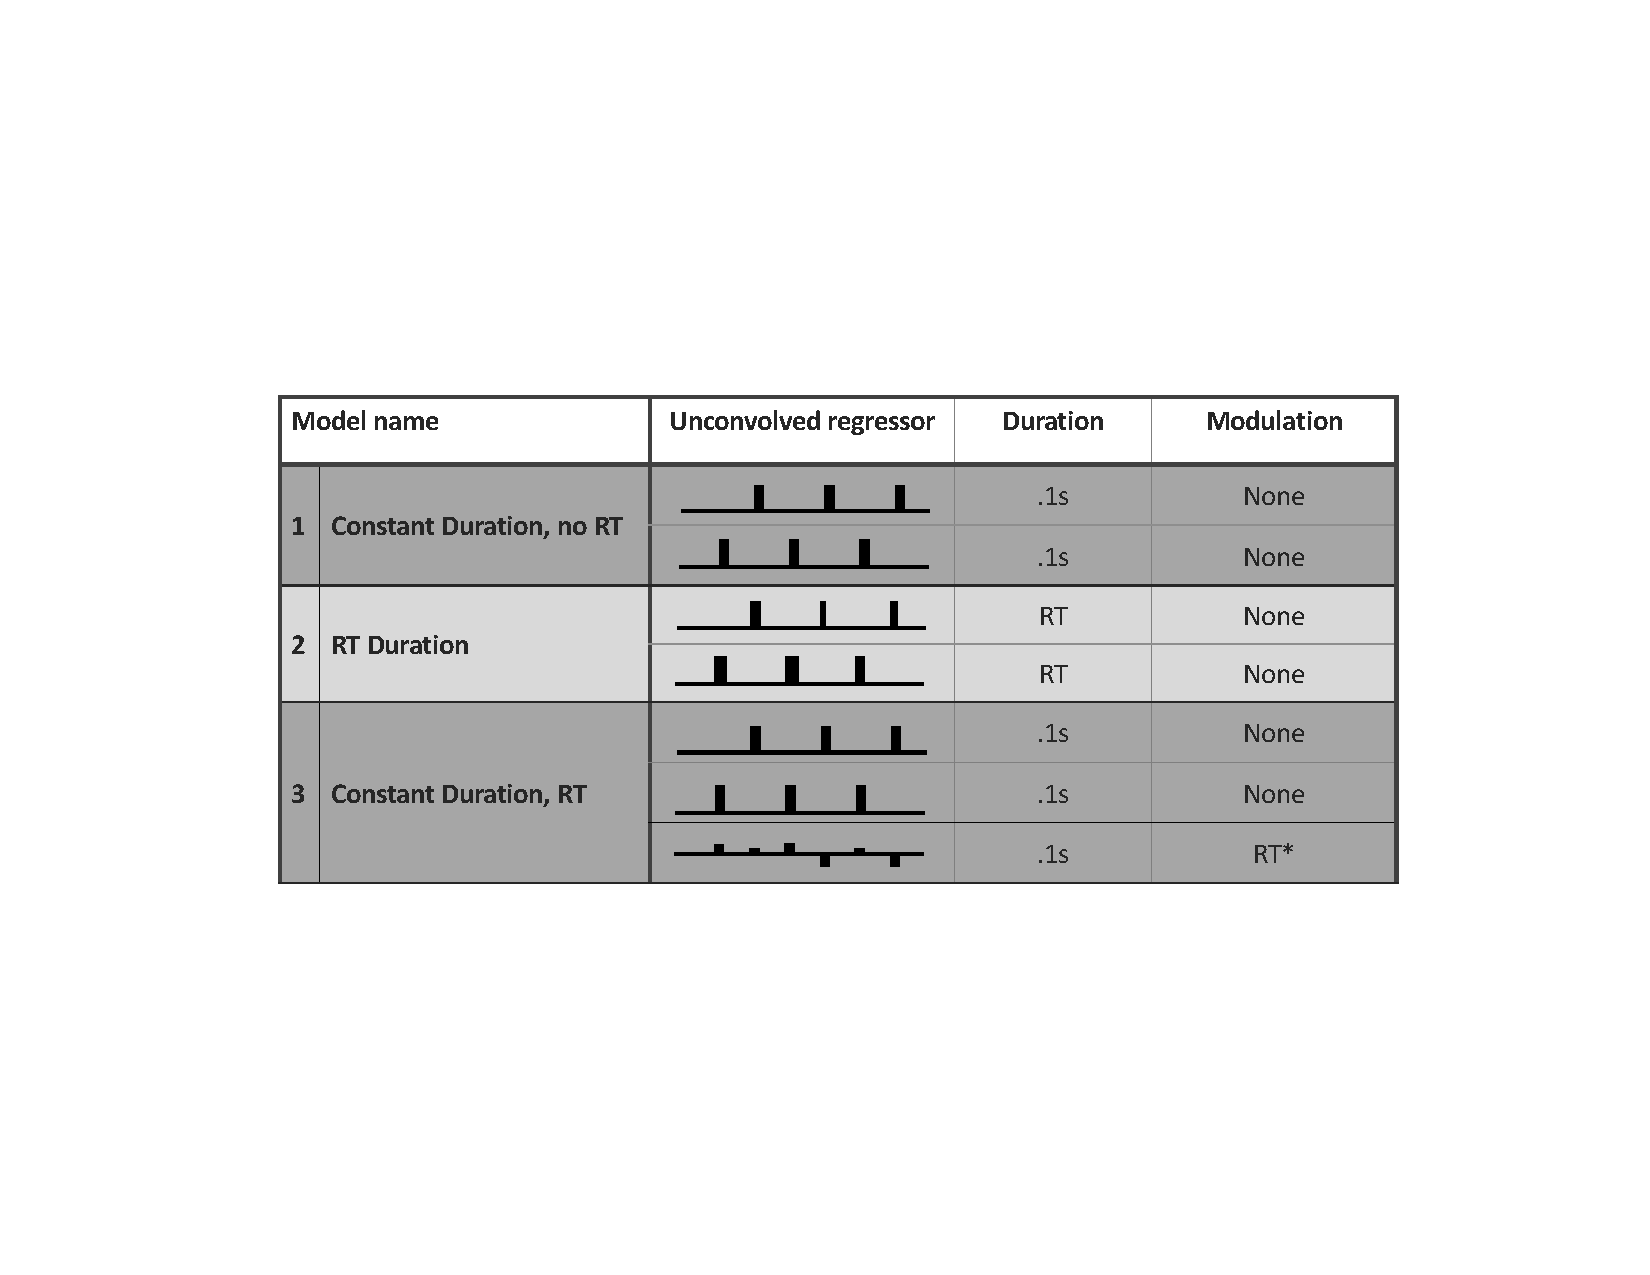
\includegraphics[width=6in]{Figures/model_explainer_2cond.pdf}
   \caption{Models assessed in the simulation study described by name, unconvolved regressor visualization, duration used for boxcars of unconvolved regressors and definition of the modulation used, when present.  Convolved regressors were used in data generation and modeling.  The first model does not include any response time information, the second model addresses RT through the duration of the regressors and the third model adds an RT modulated regressor to the first model.  $^*$See Discussion for details on why RT is not centered and other details about centering.}
  \label{fig:models}
\end{figure}

\citet{grinband_detection_2008} developed a modeling approach to address the confounding effect of response times in fMRI data, in which the duration of the boxcar function for each trial was varied by the response time on that trial (labeled as ``RT Duration'' in Figure \ref{fig:models} and hereafter as RTDur).  This approach will appropriately scale the parameter estimates for regions in which neural activity duration matches the RT duration, which we will refer to as ``the signal scales with RT''. However, the approach has two shortcomings. First, it will not correctly model activation in regions where neural activity does \textit{not} scale with RTs but rather the true duration is an unknown constant across all trials.  Second, it does not allow a separate identification of task versus RT effects; instead, it gives a composite estimate of the task effect corrected for response time.  To address these issues, we created a generalized model of RT that can identify RT effects separately from the task effect (corrected for RT); this is shown as ``Constant Duration, RT'' in Figure \ref{fig:models} and hereafter as ConstDurRT.  This model includes a boxcar function with constant duration for each of the task conditions, along with a single regressor that models the parametric modulation of the response in relation to RT for each trial. Because all RTs are modeled within a single regressor, any differences in RT between conditions will be removed by this regressor, leaving the condition difference effects to be interpreted as unconfounded estimates of activation in relation to the experimental manipulation.

Notably we have not mean centered RT or subtracted any value from RT on each trial.  This will not have any impact on the estimate of the contrast of interest (condition difference) and would only impact the condition versus baseline contrast estimate in this model.  If RT is mean centered, within run, the interpretation of some contrasts become, ``BOLD activation difference when RT is the mean RT for this run'', necessarily introducing an RT-based confound if this contrast is used as the dependent variable in higher level analyses.  This specific confound is not the focus of this work.  More details about the impact of centering RTs are included in the Discussion, including examples where it is necessary to center in some way and how to do so without introducing a new confound. For all models the effect of interest was the subtraction of condition 2 - condition 1, so the RT modulated regressor in ConstDurRT simply serves as a nuisance regressor to pick up RT variability, when present. Further details regarding the modeling approach can be found in Methods; code and data for all analyses are shared at \textbf{TBD}.

Response time data were simulated based on RTs from two different tasks: the Stroop task (based on a real data analyzed below) and a Forced Choice task used by \citet{grinband_detection_2008}.  In each case RTs were generated by sampling from an ex-Gaussian distribution \citep{Ratcliff1976RetrievalPI}; the specified ex-Gaussian parameters led to RTs that were generally longer for the Forced Choice task (mean = 1337, sd = 706.5) compared to the Stroop (mean = 690, sd = 177.5).  Another difference is that the variance relative to the mean is smaller for the Stroop task (coefficient of variation of .528 and .257 for the Forced Choice and Stroop tasks, respectively).   The interstimulus interval (ISI) was sampled from a Uniform distribution. Trials were either randomly presented conditions or blocked conditions, where 4 trials of the same condition were presented in a row.  Time series data that scale with RT were based off of the RTDur regressors and data that did not scale with RT were generated using the ConstDurNoRT regressors. 

As these analyses involve simulated data, it is likely there are features of real data that have not been incorporated into these simulations, such that some of the modeling suggestions made that remedy RT confounds perfectly in simulations may not work as perfectly in real data.  Even so, this is to be seen as a starting point to reduce the impact of this confound.  More thoughts about the remaining modeling problems will be covered in the Discussion (``How to move forward'').

\subsubsection*{Error rates and power}

We first assessed the false positive rate for each of the models on each of the simulated datasets (Figures \ref{fig:type1err_24}, \ref{fig:type1err_36}).  In all cases the ConstDurRT model appropriately controlled Type I error, but error rates were inflated when assumptions regarding the relationship between RT and neural activity were violated by the model.  Specifically, ConstDurNoRT had highly inflated error rates when activation did scale with RT, and RTDur had slightly inflated error rates when the signal did not  scale with RT.  Thus, the most commonly used model for task fMRI analysis, ConstDurNoRT, suffers from substantial inflation of false positives in the face of RT differences between conditions, because it inaccurately attributes the confounding RT signal to differences in the intensity of the underlying neuronal signal.  The larger effects observed with the Stroop-based RT reflects that the standard deviation of the RT, relative to the mean, was lower in this setting and so RT-based differences are easier to detect. The error rates for blocked designs (solid lines) are slightly higher, likely due to the fact that blocked designs have a higher signal to noise ratio, making it easier to detect RT differences in the data.  Results with a longer ISI, between 3-6s, are similar (Results shown in Figure \ref{fig:type1err_36}).

\begin{figure}
  \centering
   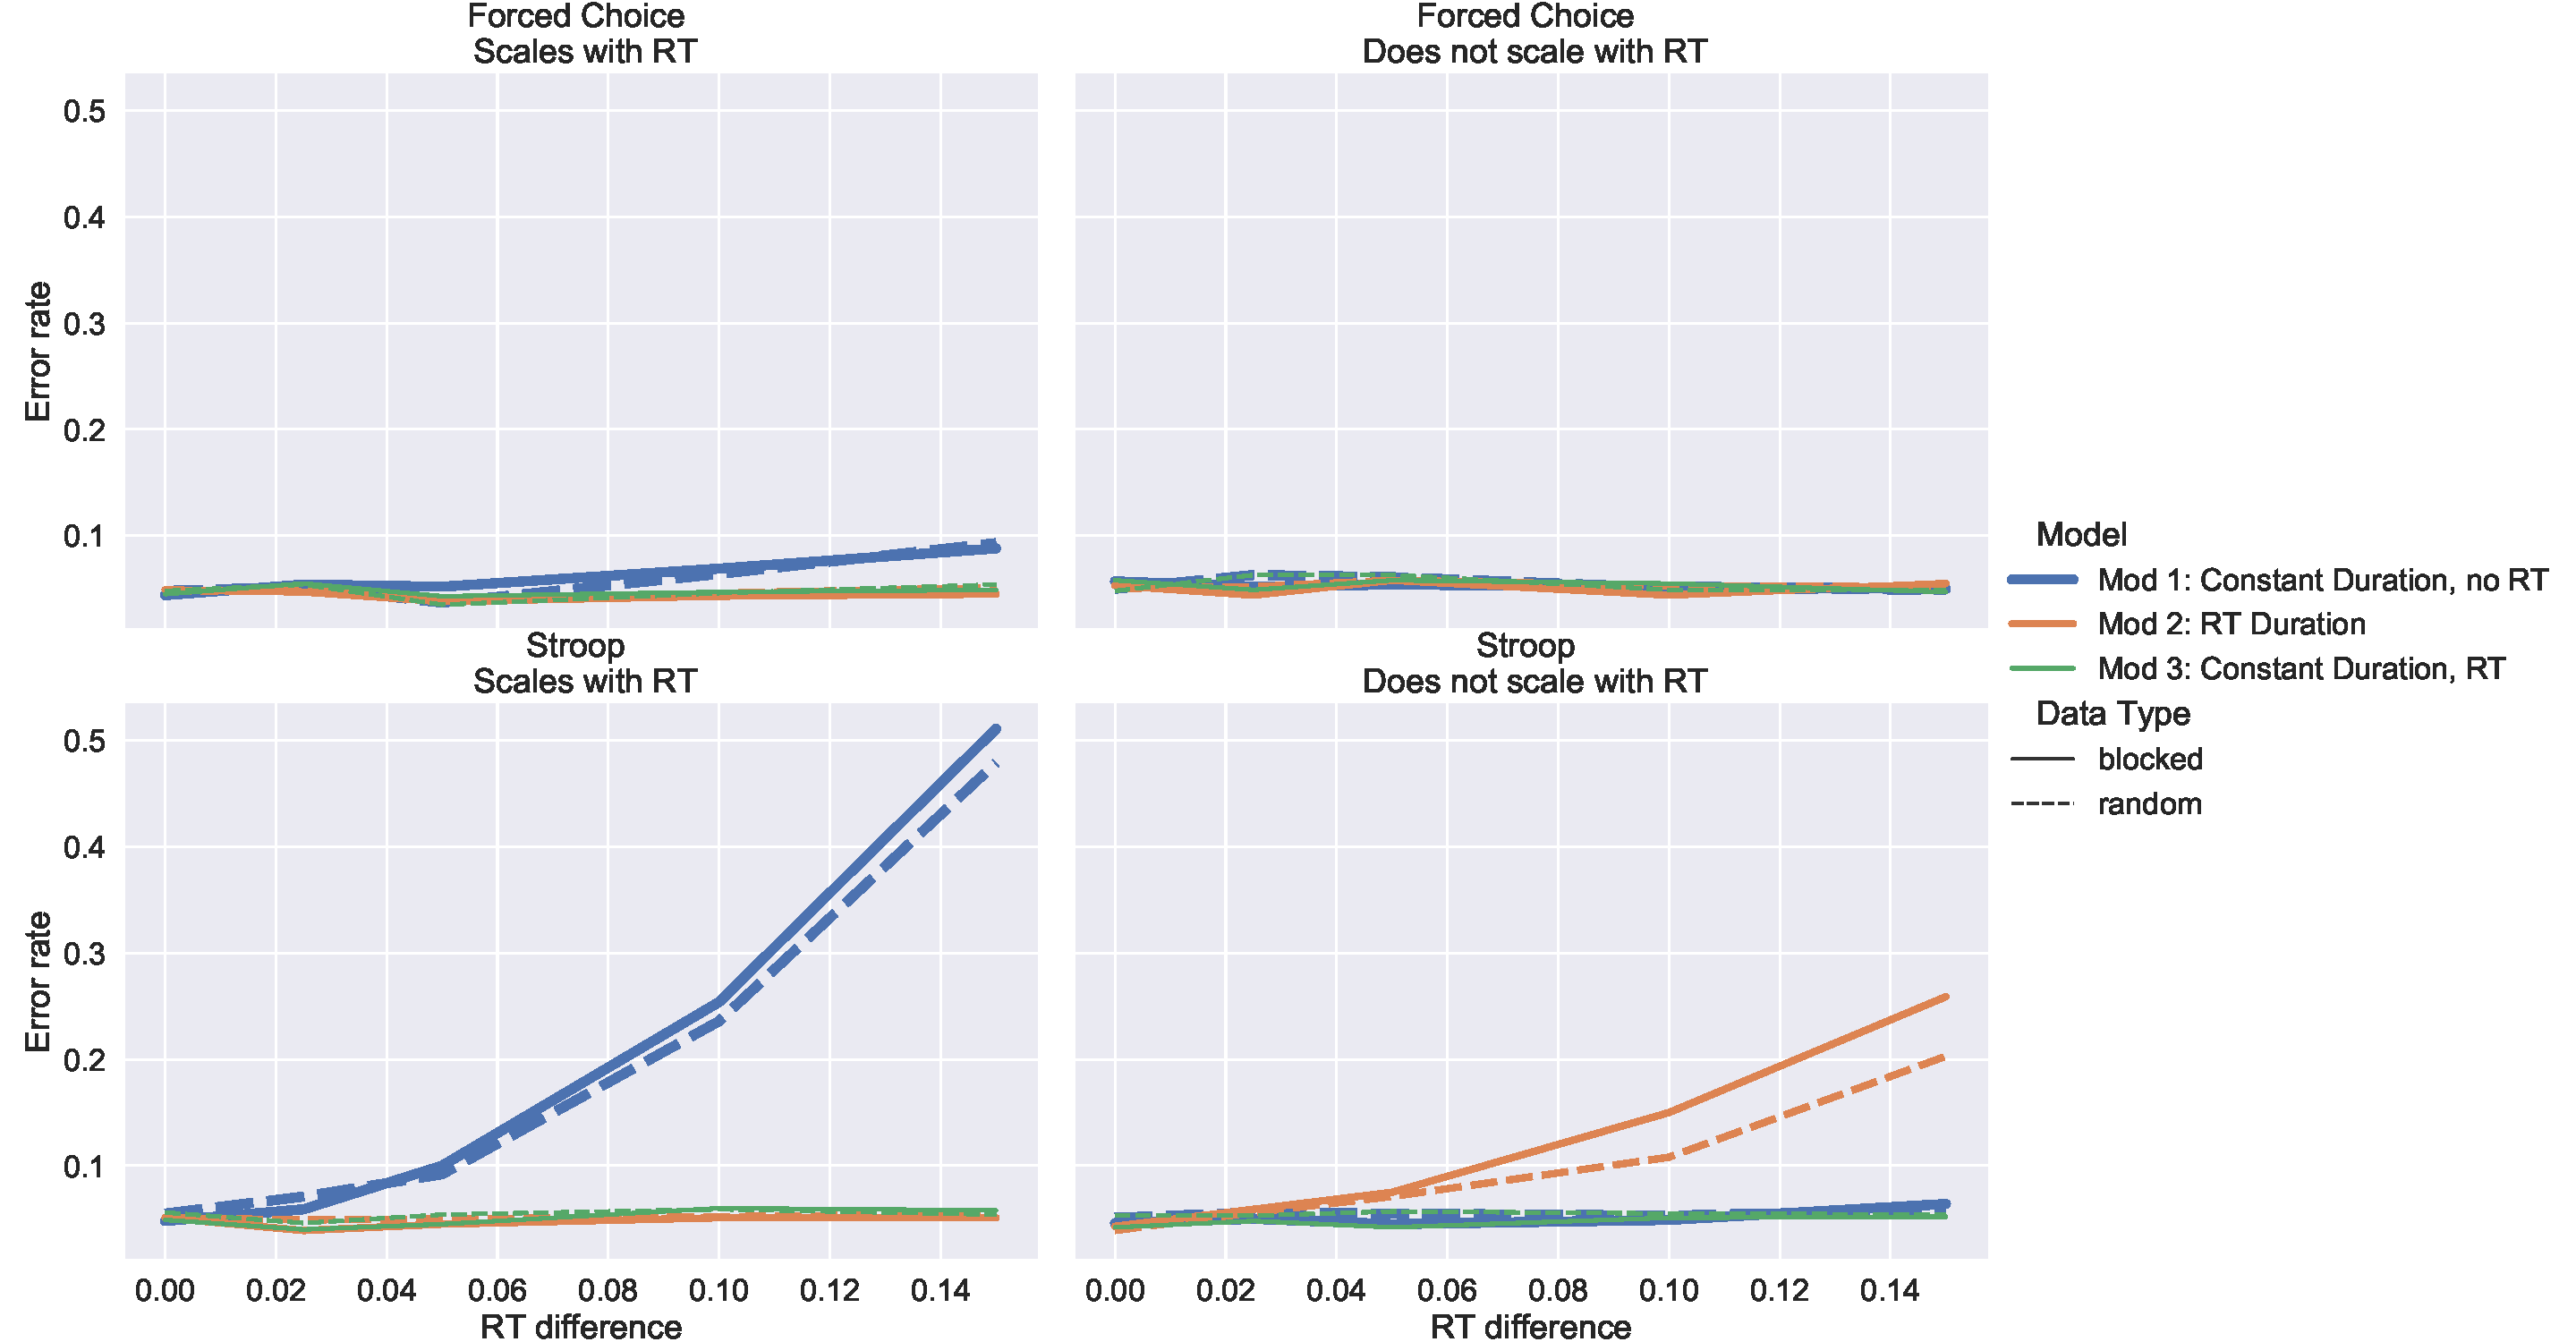
\includegraphics[width=5in]{Figures/type1_err_24.pdf}
   \caption{Type I error as RT difference between conditions increases.  The Forced Choice Task RT distribution was used in the top panels, while Stroop RT distribution was used in the bottom panels, both with an ISI between 2-4s was used and inference of interest was the 1-sample t-test of the condition effect with 100 subjects.  2500 simulations were used to calculate the error rate.  A smaller RT difference range was used for Stroop since the RT was generally shorter with lower variance.}
  \label{fig:type1err_24}
\end{figure}


It is not valid to compare the power of models that differ in their Type I error rate, so care must be taken when interpreting the power results.  We show the results for all models, but indicate which models are not valid in each scenario.  Since ConstDurNoRT is used to simulate the data when signal does not scale with RT and RTDur is used to simulate the data when the signal does scale with RT, these serve as the maximum power possible for those scenarios.  As shown in Figure \ref{fig:power_rtdiff}, the ConsDurRT model little to no loss in power in all scenarios, comparing only to valid models.  The seeming increase in power for ConsDurNoRT is biased by RT and, interestingly, the RTDur model shows a large loss in power when the signal does not scale with RT due to the model strictly trying to fit an RT effect that is not present.  As the true model is unknown in real analyses, this establishes that ConsDurRT is a flexible model that can adjust to whether the signal scales with RT,  assuaging concerns that using ConstDurRT will result in power loss for within-subject condition versus baseline effects, as suggested by \citet{grinband_detection_2008}.  


\begin{figure}[h!]
  \centering
   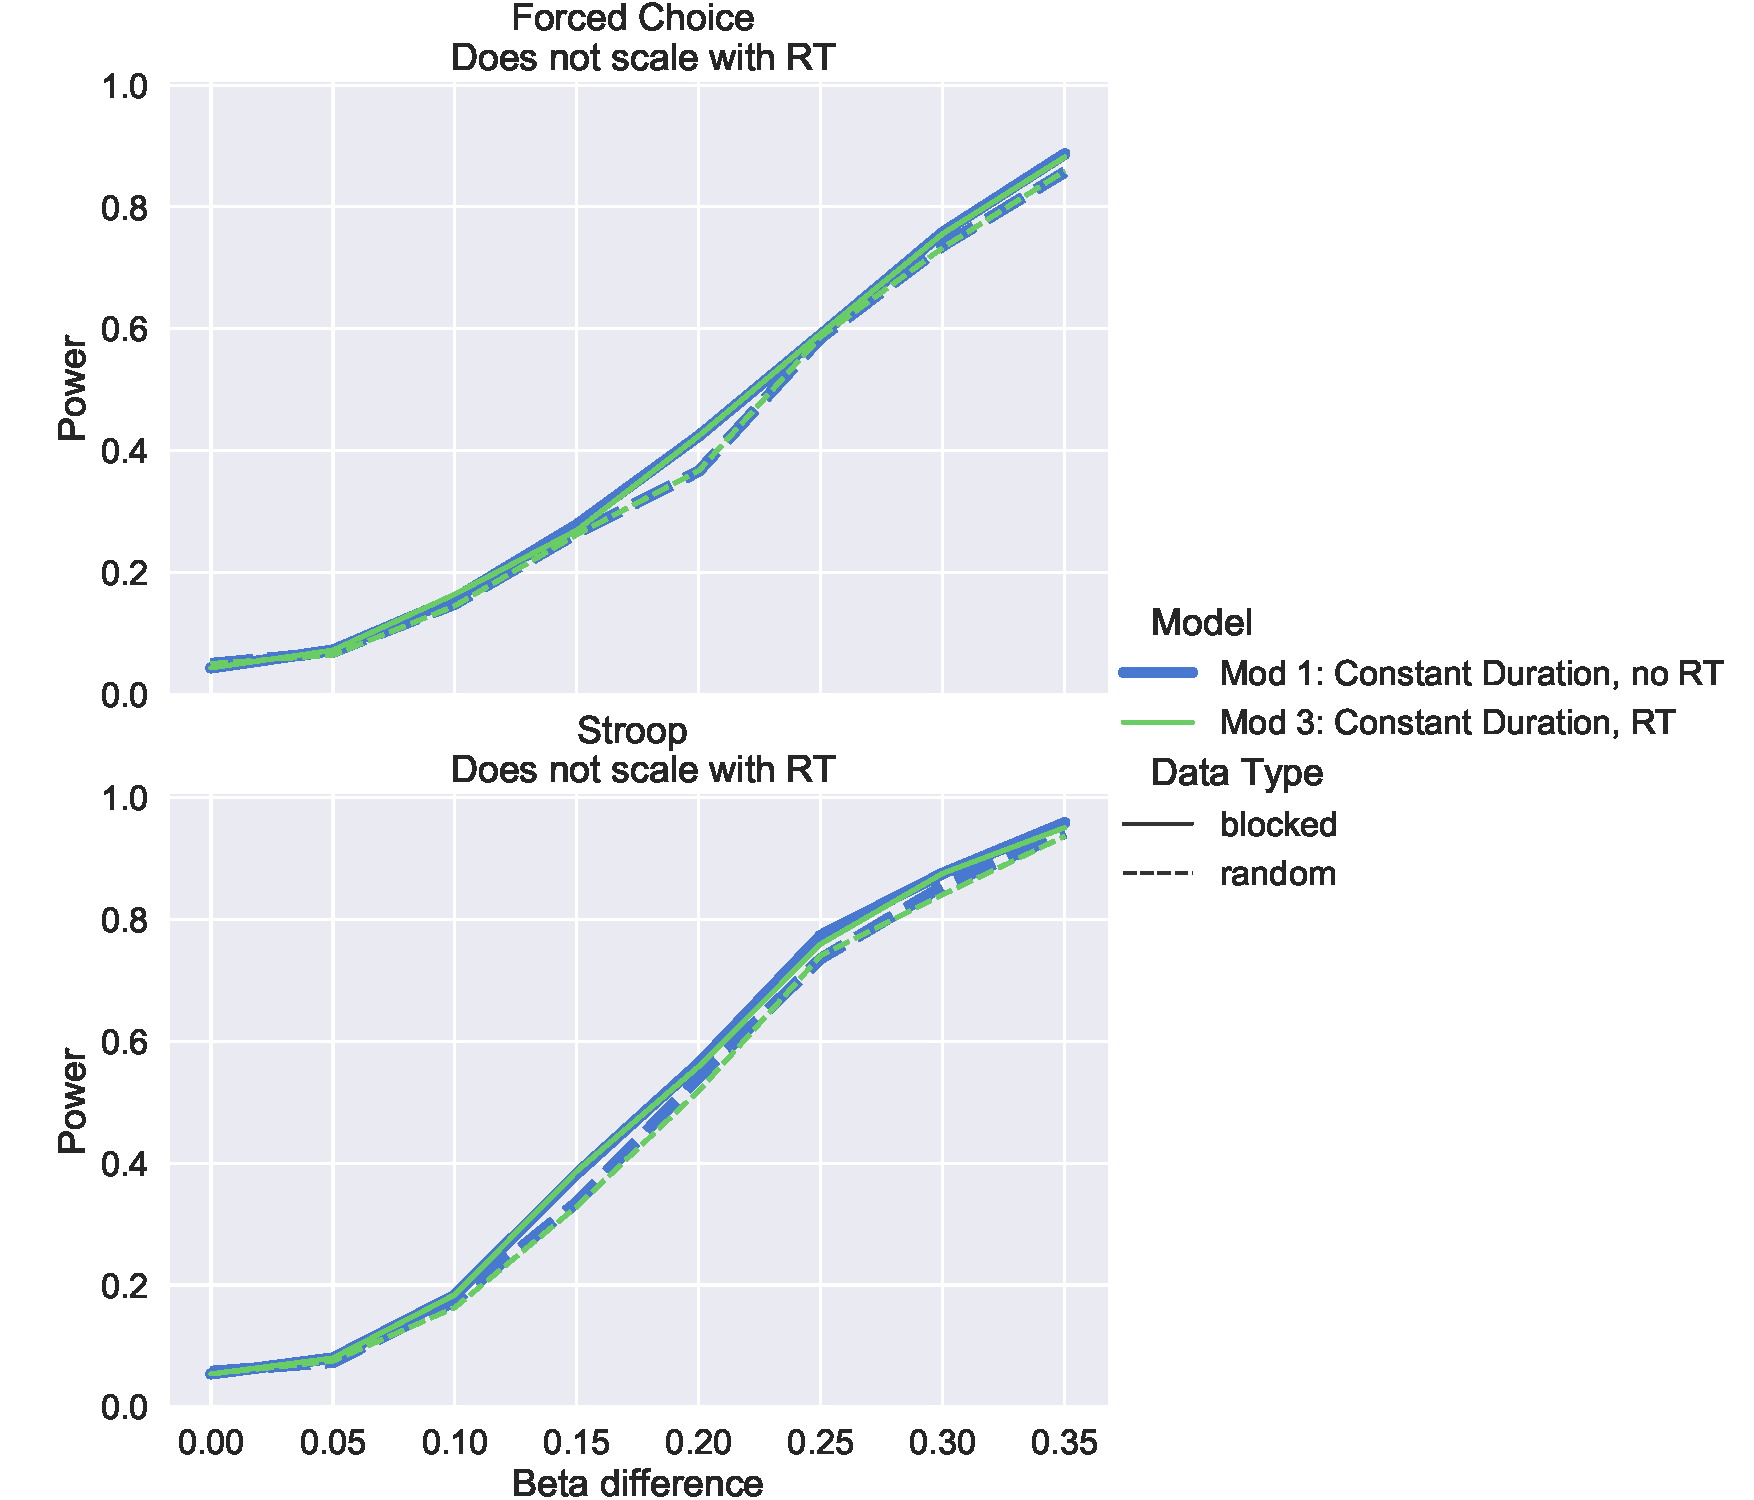
\includegraphics[width=5in]{Figures/power_24_rtdiff_1.pdf}
   \caption{Power when RT difference is 0.1s as the condition difference increases. Power for all models is shown, although cannot be interpreted for models that did not control Type I errors as they are invalid.  When signal scales with RT (left panels) RTDur is the true model and will have maximal power (orange), while ConsDurNoRT is invalid (blue). When signal does not scale with RT (right panels) the true model is ConsDurNoRT (blue lines) while the RTDur model is invalid (orange). In all cases the ConsDurRT model has comparable power to the true model.  Sample size is 100, with an ISI between 2-4s. }
  \label{fig:power_rtdiff}
\end{figure}


\subsection*{Correlation of condition contrast with condition differences in RT}

The foregoing analyses, along with the previous work by Grinband, focused on confounding of RT between-trials, which impacts average condition effects.  Here we introduce a new problem of a between-\emph{subject} RT confound.  The within-subject differences in average RT, corresponding to the contrasted conditions,  can confound group level analyses involving group comparisons or associations.  This is of particular interest given the increasing focus on analysis of brain-behavior correlations in fMRI literature (e.g. \citet{duboisBuildingScienceIndividual2016}).

The driving factor of correlations between condition differences in brain activation and the corresponding differences in RTs is easy to understand due to a simple linear relationship between the activation estimate and RT when the data and model assumptions are in conflict. In the case where signals scales with RT and the ConstDurNoRT model is used (duration = 1s), the relationship between the estimated activation, $\hat\beta$, and the true activation, $B$, is approximately $\hat\beta = B \times RT$, for a single trial.  Figure \ref{fig:rt-cor} shows this linear relationship holds within the range of RTs one would expect to observe in most data sets.  Moving from the activation estimate of a single trial to the BOLD activation across multiple trials, the relationship becomes $\hat\beta = B\times \overline{RT}, $ where $\overline{RT}$ is the average RT across trials.  Last, for two conditions, $1$ and $2$, assuming $B$ is a common true activation, the relationship for the contrast of conditions is $$\hat\beta_1 -\hat\beta_2 = B\times\left(\overline{RT}_1 - \overline{RT}_2\right).$$
From this it directly follows that at the \emph{group} level there is an expected linear relationship between the estimated condition difference and the difference in RTs, specifically the between-subject slope would be $B$, the true, common activation of the two conditions.  Notably, this linear relationship does not require a non-zero RT difference on average, but simply between-subject RT variability; therefore the RT difference is an important confound regardless of whether it is significantly different from 0 on average.

\begin{figure}
  \centering
   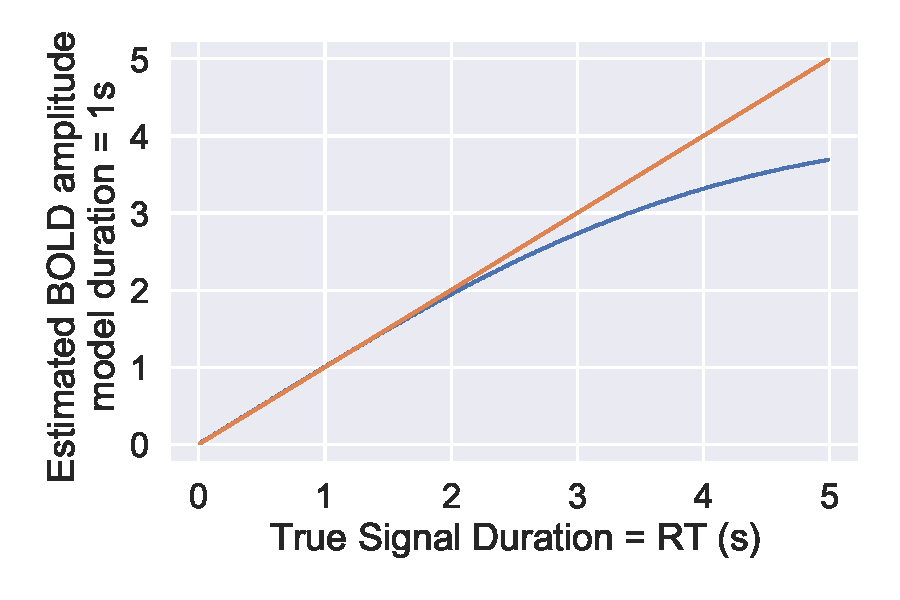
\includegraphics[width=3.5in]{Figures/bold_fcn_rt_1sdur_only.pdf}
   \caption{Relationship between trial RT and the trial-specific BOLD activation estimate when a constant duration of 1s regressor is assumed and signal scales with RT.  The true BOLD activation is 1, but the model estimates the BOLD activation to be $1\times RT$ for RTs $<$ 2s. \textbf{need to define the red and blue lines, and/or (better) include a legend in the figure}}
  \label{fig:bold_rt}
\end{figure}


The simulation results in Figure \ref{fig:rt-cor} show the relationship across all models and data types considered in this work, repeating the relationship described above where the signal scales with RT and ConstDurNoRT is used as well as illustrating the RtDur model has a similar issue when the signal does not scale with RT.   Notably, the data were simulated such that the variance in RT did not change with RT, whereas in real data the variance of RT often increases with its mean.  The implication is the correlation estimated by our simulations is conservative.  Even so, it is within the ballpark of the expected true correlations between brain and behavior measures \citep{marekReproducibleBrainwideAssociation2022}.  

\rh\ph\textbf{(Within the following paragraph I describe a real data analysis (Figure S3) can you help me with brain anatomy descriptions/interpretation?)} 

In a real group level data analysis of the Stroop task, we show significant correlations between the incongruent versus congruent contrast estimate and the corresponding RT differences when using the ConstDurNoRT time series model  (Figure \ref{fig: group_corr_stroop}); no significant relationships are found in the same group level analysis when the ConstDurRT time series model was used (N=98).  Given this, adjustment for RT in higher level analyses is important when using the ConstDurNoRT or RTDur models.  For contrasts that are more complicated than a simple difference between two conditions, one can add a separate mean RT confound for each condition involved in the contrast in the group level model.


\begin{figure}
  \centering
   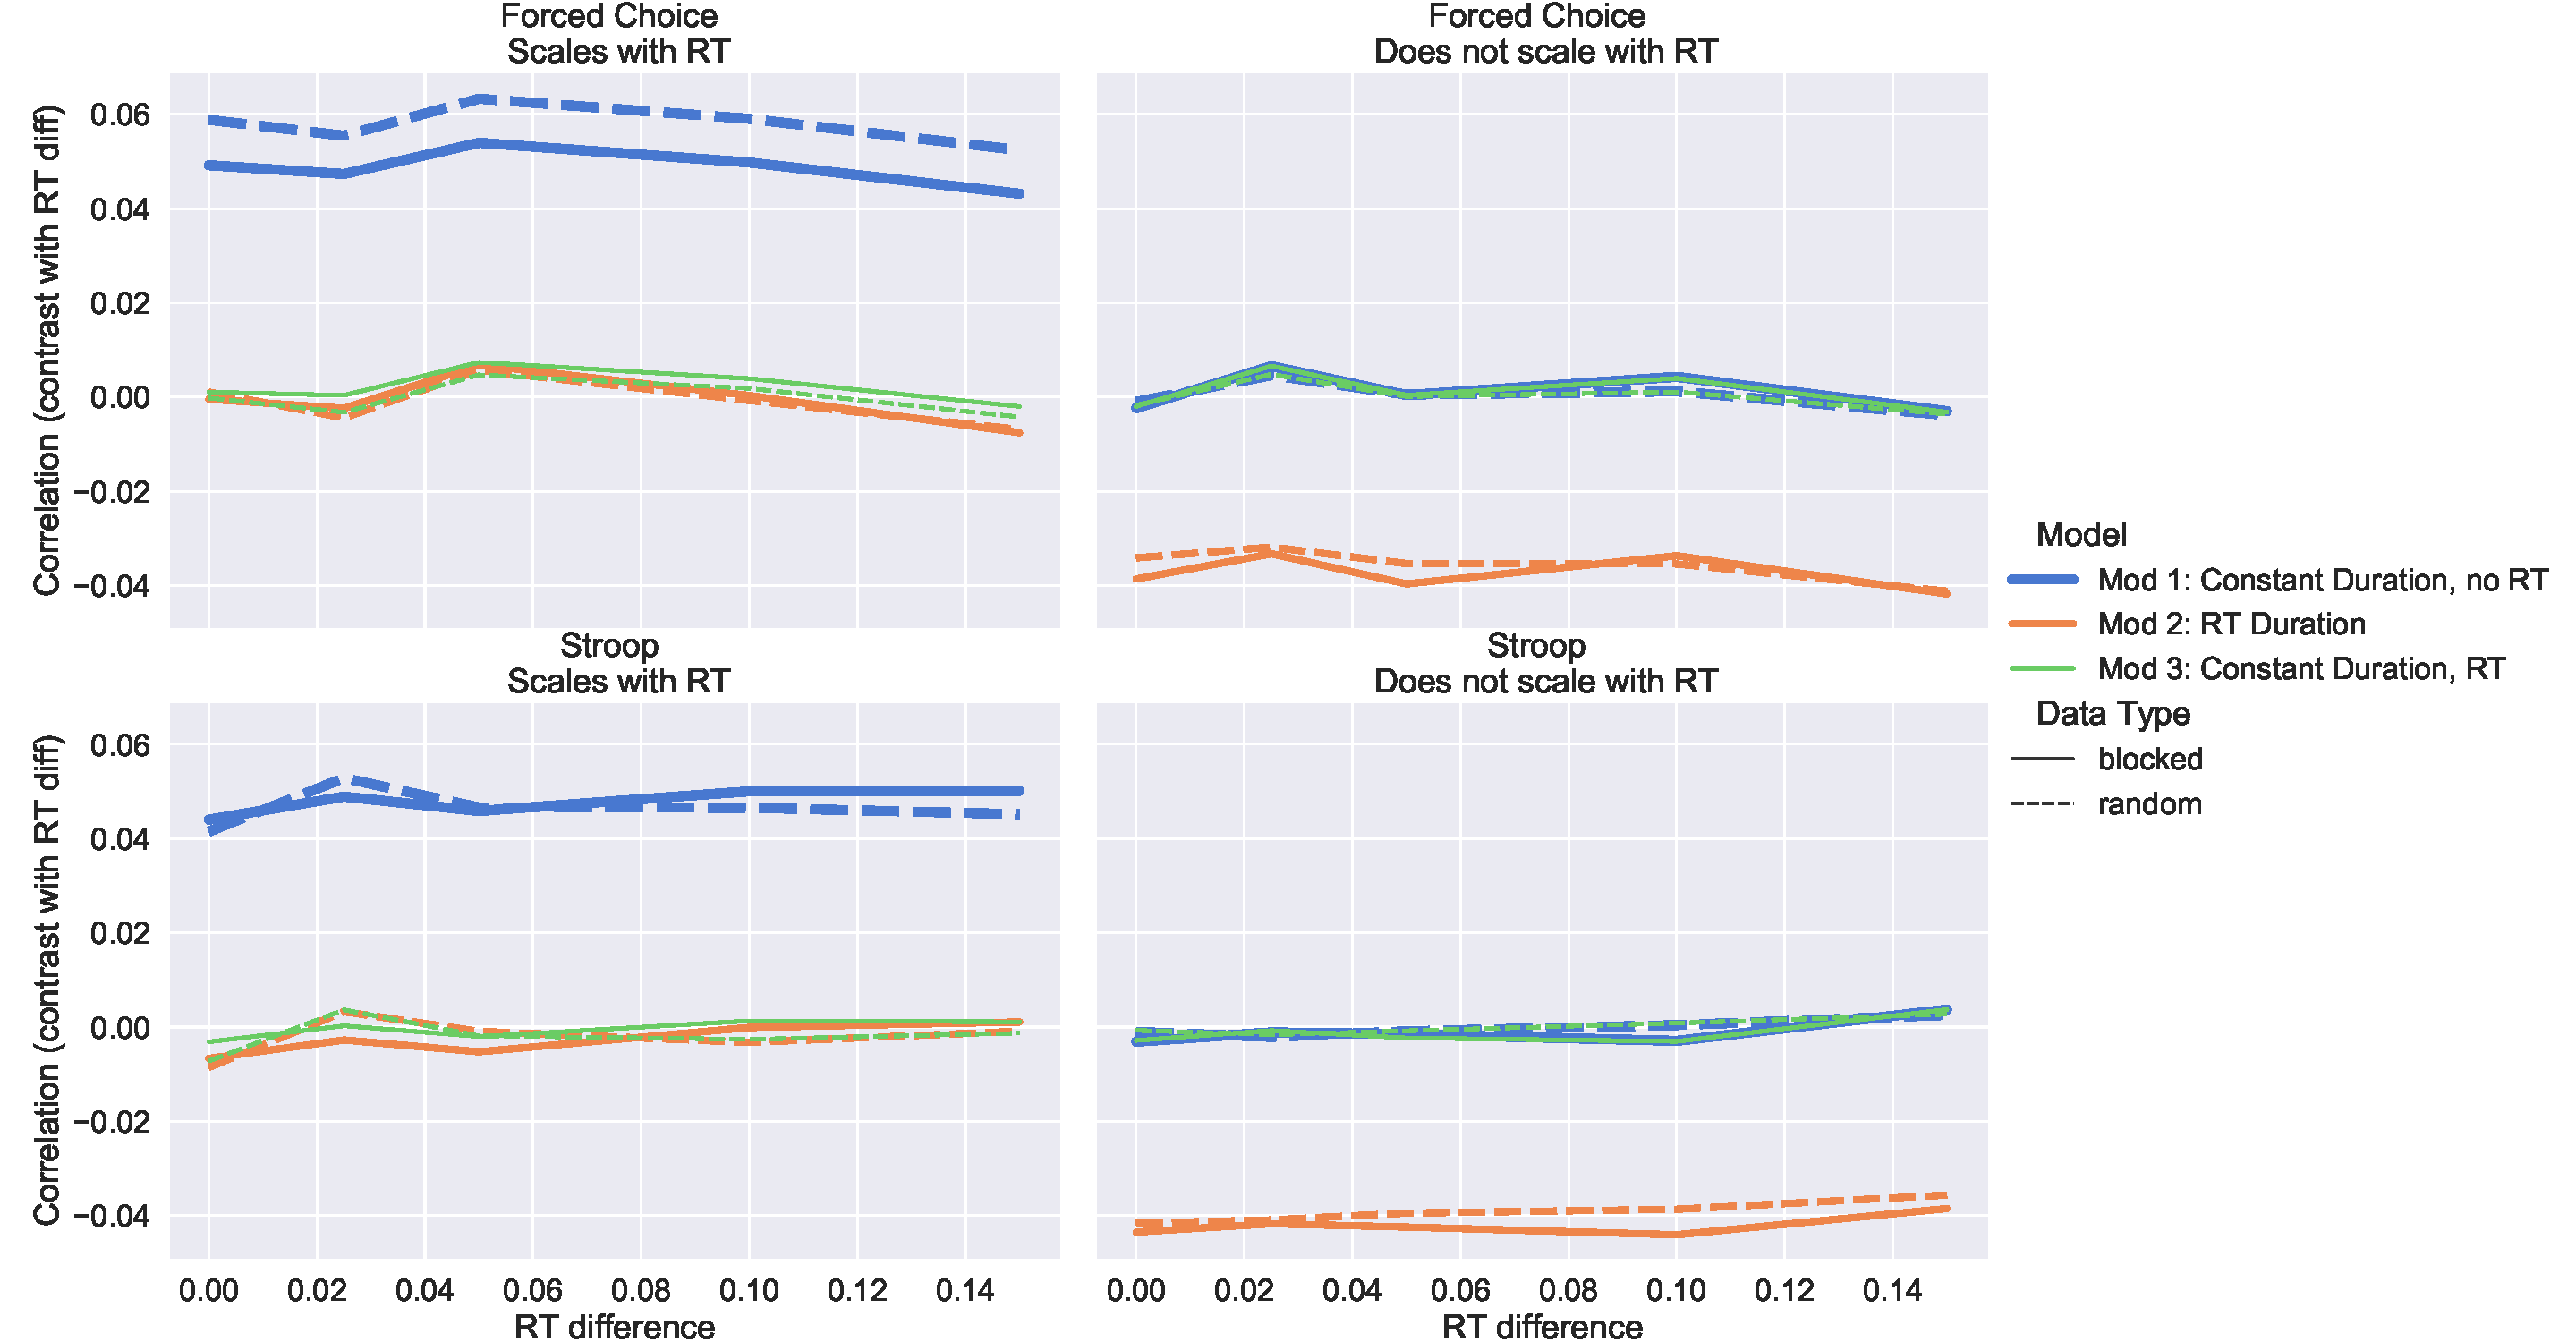
\includegraphics[width=5in]{Figures/cor_with_rt.pdf}
   \caption{Correlation between the contrast difference and difference in average condition RT across subjects as a function of the average difference in RT between conditions.  Since the correlation is driven by between-subject variability in the \emph{difference} in RT, there is no requirement that RTs differ between tasks and the correlation is constant regardless of the RT difference. }
  \label{fig:rt-cor}
\end{figure}




\subsection*{Widespread RT activation is not specific to task, revisited}

\ph\rh\textbf{(In the following, is it possible to write a sentence with a short blurb about what each task is tapping into?  I have details in the supplement, but they're the long descriptions you pointed me to earlier.  If they do not overlap in terms of function that is being measured and if these are different from Yarkoni's tasks of working memory, emotion, and decision making, it is worth mentioning.  It is especially important to describe how any of these tasks are different from stroop.  My goal is to establish that it isn't likely that the common activation is due to some overlapping psychological event that all of these tasks tap into.  For example, could somebody argue that all of these tasks reflect conflict (or something similar) and that's why there's so much overlap?)} 

\textbf{ This set of tasks is certainly less diverse than the tasks that Tal used in his paper - some of these are fairly similar to stroop (e.g. ANT, DPX) while others (DDT, stop signal} are rather different.}

Our real data analyses were modeled to included separate regressors for each condition as well as a single RT regressor to control for RT effects in our contrasts between conditions, similar to the ConsDurRT model.  A total of 7 tasks, each with approximately 96 subjects, were analyzed.  Brief descriptions are given in Table \ref{tab:task_summaries} and more details summaries are provided in the Methods section.   The focus here is on the RT-related effect.  Notably, this effect estimate will be slightly diminished from a full RT effect, since it is adjusted for condition difference and so the interpretation would be the average within-conditon RT effect. Group statistics maps were thresholded using the TFCE p-value (from FSL Randomise) less than 0.05 with 5000 permutations.  The conjunction, in Figure \ref{fig:conj} shows voxels where the RT-modulated effects were significant across all 7 tasks.  This is an updated version of the maps shown in \citet{yarkoni_bold_2009}, which used 2 3-back tasks, decision making, emotion ratings and memory in sample sizes of 50, 102, 26, 35 and 39.  Our maps are consistent with those, but with a more spatially widespread effects, which may reflect the fact that our analysis uses a within-subject comparison. In particular, the present comparison demonstrated substantially more signal in the lateral superior parietal cortex \rh \ph\textbf{(can somebody look at the maps from Yarkoni and help me compare?  Figure temporarily inserted here, see Fig \ref{fig:conj-yarkoni})}

\begin{table}[h!]
  \begin{center}
    \caption{fMRI task summaries \textbf{(Under construction, N's will change with final analyses)}}
    \label{tab:task_summaries}
    \begin{tabular}{|L{6cm}|L{7cm}|L{1cm}|}\hline
   \textbf{Name} & \textbf{Description} & \textbf{N} \\ \hline\hline
   Attentional Network Test (ANT) &  Tests three attentional networks: alerting, orienting, and executive control & 99 \\ \hline
   Kirby Delay-Discounting Task (DDT) & Measure of temporal discounting, the tendency for people to prefer smaller, immediate monetary rewards over larger, delayed rewards & 88 \\ \hline
   Dot Pattern Expectancy (DPX) & Measure of individual differences in cognitive control & 96 \\ \hline
   Motor Selective Stop Signal & Measures the ability to engage response inhibition selectively to specific responses & 99 \\ \hline
   Stop-Signal Task & Measure of motor response inhibition & 100 \\ \hline
   Stroop & Measure of cognitive control & 98 \\ \hline
   Cued Task-Switching Task (CTS) & Indexes the control processes involved in reconfiguring the cognitive system to support a new stimulus-response mapping & 101 \\ \hline
    \end{tabular}
   \end{center}
 \end{table}

\begin{figure}
  \centering
   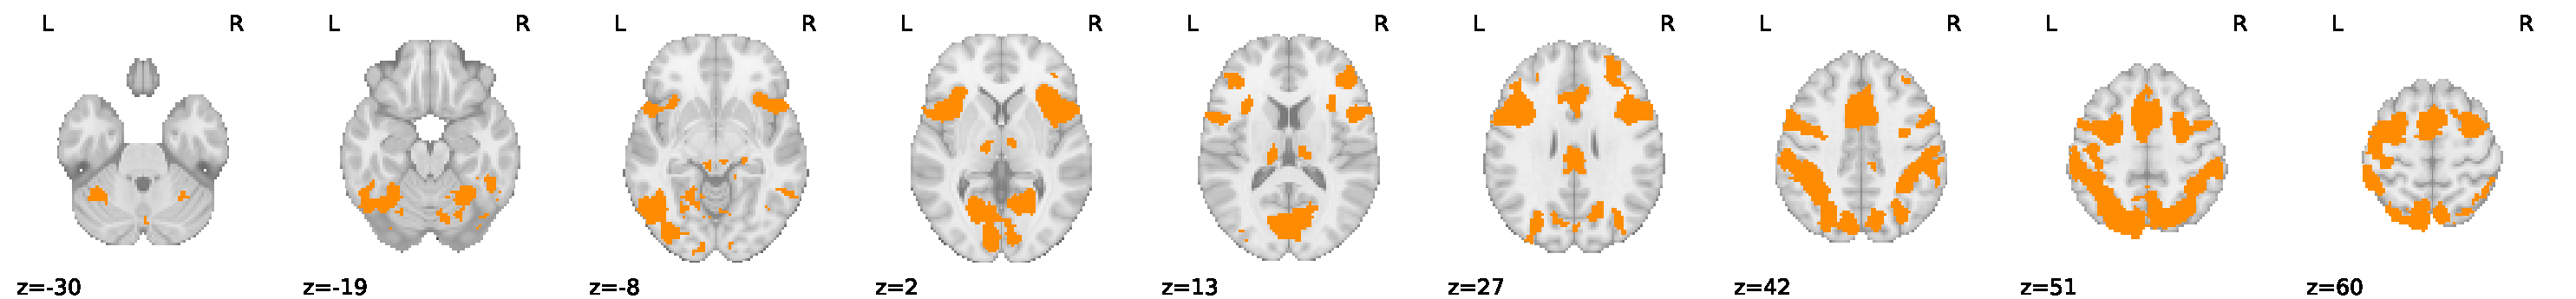
\includegraphics[width=6.5in]{Figures/conjunction_avg_rt_effect_across_7tasks.pdf}
   \caption{Conjunction of the average, within-condition RT effect across ANT, DDT, DPX, motor selective stop, stop signal, stroop, and CTS.  On average, each analysis included 96 subjects and maps were corrected for multiple comparisons using a TFCE p-value thresholded at 0.05 using 5000 permutations.}
  \label{fig:conj}
\end{figure}


\begin{figure}
  \centering
   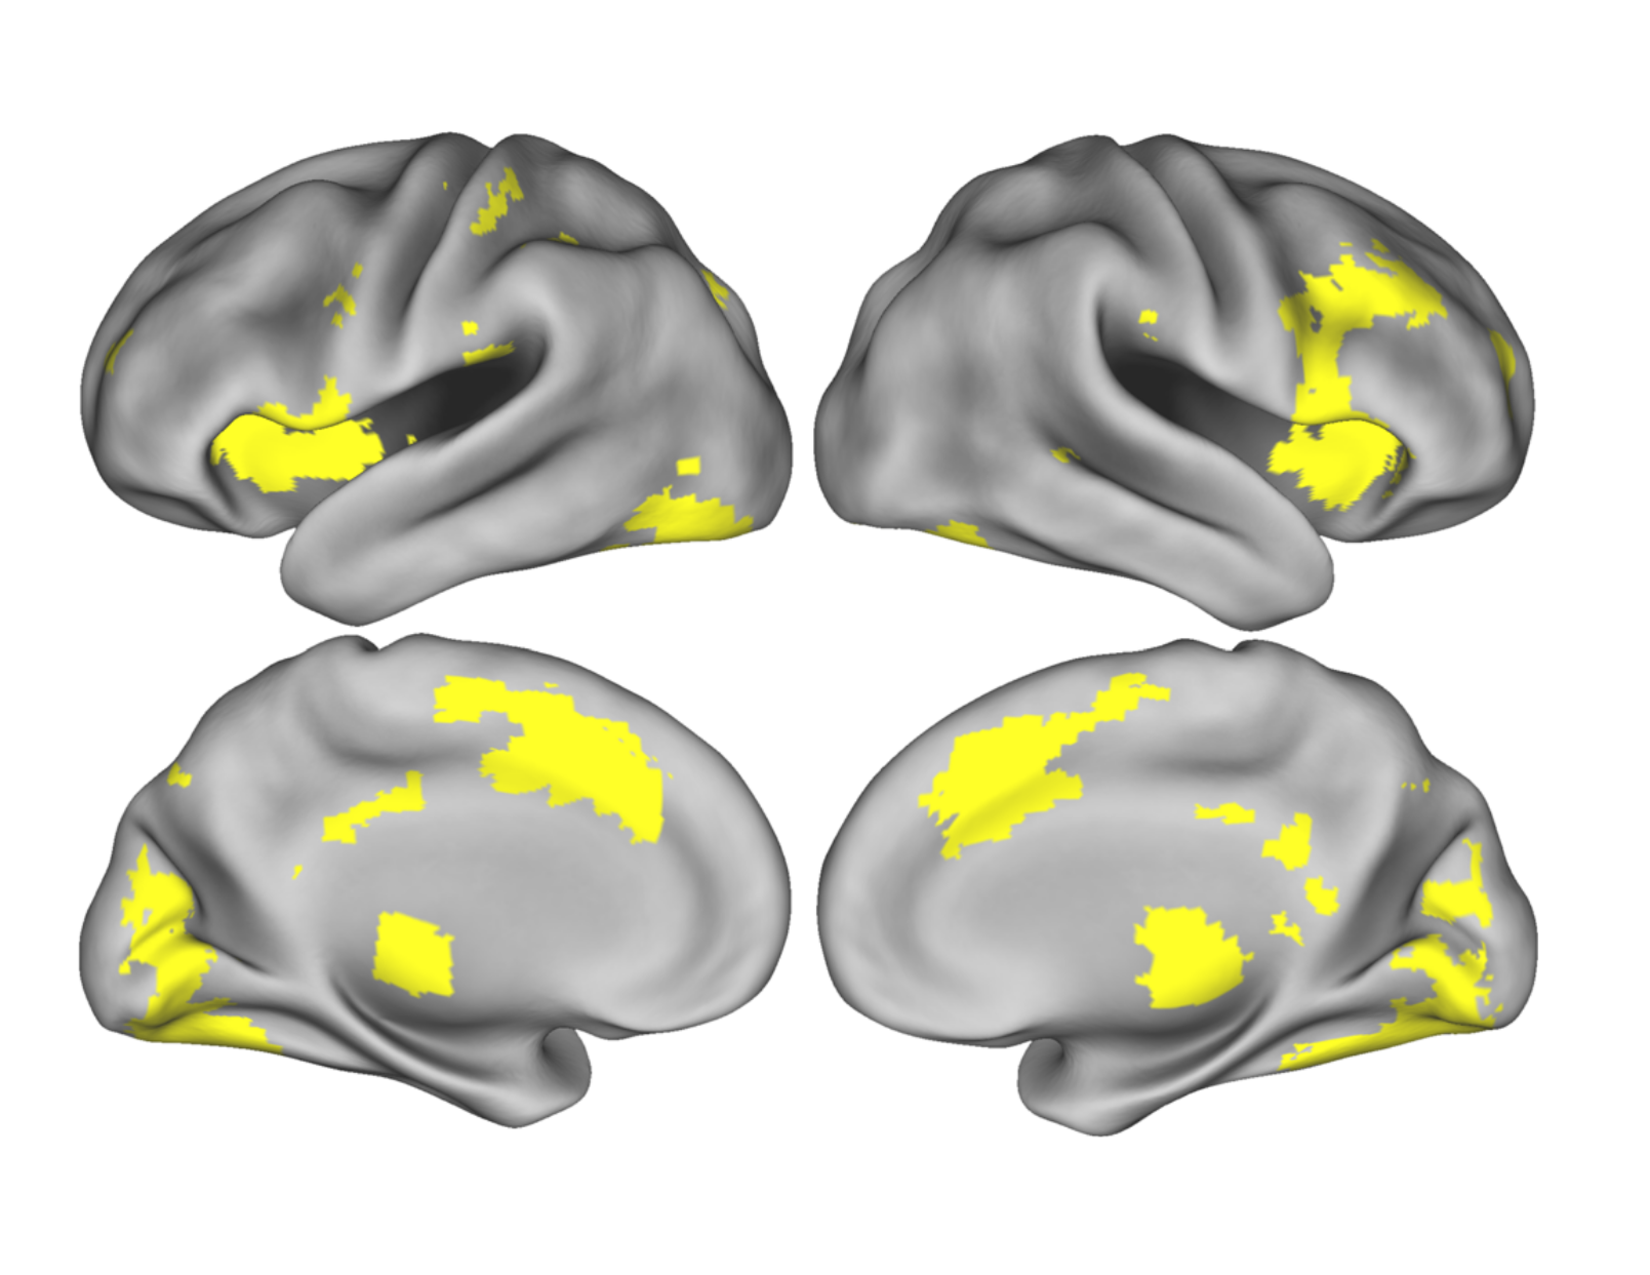
\includegraphics[width=4in]{Figures/temporary_fig_from_yarkoni.pdf}
   \caption{TEMPORARY.  This is the figure from Yarkoni for comparison during revisions. From that paper: Figure 2. Cortical regions that showed significant RT-related activation in all five samples. Clockwise from top left: ,left lateral, right lateral, left medial, and right medial views of the cortical surface. doi:10.1371/journal.pone.0004257.g002}
  \label{fig:conj-yarkoni}
\end{figure}


\section*{Discussion}

The problem of potential response time confounds for fMRI activation estimates has been discussed for more than a decade, but there has been little resulting change in how the community approaches analyzing and interpreting fMRI contrasts when RT differences between task conditions are present.  There are three takeaways from the present work.  First, we propose a modeling approach that more effectively adjusts within-subject contrast estimates for response time differences, so that group average estimates of contrasts are adjusted for between-condition response time differences.  Second, this work highlights an important problem that has not been discussed previously: 
the presence of a between-subject analysis confound of the average RT differences.  Finally, we replicate previous work showing that RT-related effects are not task specific and the effects are widespread, using more tasks with larger sample sizes than used in \citet{yarkoni_bold_2009}.

This work presents a model that can adapt to data whether or not the signal scales with RT, without losing performance. By adding an RT modulated regressor to the most commonly used model that only contains condition-specific regressors, the ConstDurNoRT model reduces RT-driven type I errors in average condition comparison effects without a reduction in power.  The commonly used ConstDurNoRT model assumes the signal does not scale with RT and the RTDur model assumes the signal must scale with RT, hence both models fail to control error rates when these model assumptions are violated (Figure \ref{fig:type1err_24}).  


We have also uncovered that subject-specific differences in average RT represent an important group-level confound.  This confound is only present if the time series model follows the ConsDurNoRT or RTDur approaches, whereas the ConsDurRT model produces condition difference effects that are free of this confound.  Notably, the average difference in RT across subjects does not impact the strength of the correlation, since the correlation is driven by the variability in RT differences across subjects.  Thus, even if the RT difference is 0, on average, one should still include the RT adjustment in group analyses when using ConsDurNoRT or RTDur time series models.


Last, our updated RT-effect conjunction analysis across 7 tasks tapping into different mental processes show widespread shared activation in the so-called ``task-positive'' network, replicating the previous results of \citet{yarkoni_bold_2009}. This highlights the generality of the RT effect across tasks, and motivates the need to model these effects across all tasks.  The presence of the aforementioned group-level confound suggests that this should be done whenever brain-behavior associations are of interest, even when there is no mean difference in response times across conditions.

\subsection*{The paradox that RT is the effect of interest in fMRI studies}
\rh\ph \textbf{(please verify that I am not overstating in the interpretations of the Grinband or Yeung papers below)}

Since RT differences are the measure of interest in behavioral studies, there is widespread resistance to treating RT as a confound in fMRI models, as we recommend here.  A common argument is that RT is the measure of interest and not a nuisance covariate in fMRI models.  However, this idea is in conflict with the models typically used.  Using the Stroop task to illustrate this paradox, recall that \citet{grinband_dorsal_2011} concluded the Stroop effect was reflecting time on task, as similar activation patterns for incongruent versus congruent trials were found when contrasting slow and fast congruent trials.  \citet{yeung_errors_2011} attempted to refute this argument by arguing that slow congruent trials are reflective of increased conflict.  A first problem with this argument is that it implies that one should use RT as a proxy for conflict rather than rather than the congruency manipulation that is commonly used as a proxy for that cognitive process.   In this case a more powerful model would be to \emph{replace} the two condition effect regressors  with a single RT-modulated effect and then this RT effect would be the effect of interest.  This raises a second problem with this logic, since the resulting activation pattern would look like our conjunction effect in Figure \ref{fig:conj}, which included Stroop-based RT effects as well as six other tasks, suggesting that the process of interest is so nonspecific as to be of limited utility for understanding brain function.   It seems more useful to instead study the task effect, adjusted for RT, and RT effects in parallel to obtain a condition effect that is not biased by RT and also to isolate the RT-based activation in an effort to better understand what it reflects in the data. 

\subsection*{Modeling considerations}

\subsubsection*{Should the RT modulation values be centered?}
We did not center RT in our models, as it would not have any impact on the condition difference estimate since trials in both conditions involve RTs and the model implies the same condition difference effect occurs for all RTs.  A common practice is to center by the mean RT for that subject and run of data, but this can introduce RT information into some contrast estimates.  For example, if RT is centered, the interpretation of a condition versus baseline effect is specifically for that subject/run's mean RT.  In this case there is an obvious RT confound introduced at the group level since each subject's activation reflects their own RT.  The same will occur for any contrast where one condition involves RTs and another does not.  For example, in the stop signal task the go trials have a response time whereas successful stop trials do not.  Therefore if RT is centered within-subject and run, the go versus successful stop contrast estimate corresponds to the magnitude of the effect for mean RT of that subject/run, such that a correlation between this contrast and the average go RT will leak into the group level analysis.

There are two options in the case where some contrast comparisons involve a mix of conditions that do and do not have RT effects.  If RTs are mean centered, then the mean RT regressors must be added to group level analyses, as described below.  An alternative is to simply center by the same value for all subjects and runs.  This value can either be the mean RT across \emph{all} subjects and runs or a value that is roughly what one would expect the average RT to be for that task.  In this case the RT confound at the group level should not be present.  If all condition comparisons involve conditions with RT effects, then centering RT in the modulated regressor will have no effect on the contrast estimates of interest.



\subsubsection*{Avoiding common pitfalls when adding RT to a time series model}
When adding RT to the time series model, there are some  common mistakes that should be avoided.  Most of the problem relates to the intuition that collinearity between regressors is bad and mean centering or orthogonalization is always necessary.  Once the data have been collected and the models are set up, collinearity with regressors of interest often cannot be resolved, but may have been preventable with a different study design.  In the case of RT, if the RT regressor is highly collinear with the task contrast, this should not be altered, by orthogonalization or centering RT within task, as that obviates the motivation for adding RT in the first place: controlling condition differences for RT differences or time on task effects.  If RT is mean centered within-condition, then it is misleading and incorrect to claim the condition effects have been adjusted for RT differences.  If RT is split into separate regressors by condition, this model implies an interaction effect between condition and task is suspected.  In this case, if the interaction is significant, then that is the contrast that should be studied in detail as it indicates the magnitude of the condition difference varies by  RT.  Our recommendation is if there is not an expected interaction between different conditions and RT, then a single RT regressor should be used.  


\subsubsection*{How to adjust for the RT confound in group level analyses}

The contrasts used in the simulations above were simple differences between two conditions, but other contrasts may be more complex.  A general, flexible approach for removing RT confounds in higher level analyses, is to  add a single average RT regressor for \emph{each} condition involved in the contrast in the group level model.  For example, if positive, negative and neutral conditions for a task were combined in a contrast estimate at the time series level, one would add three RT regressors to the higher level analysis: the mean RT for each of positive, negative and neutral trials.  This will provide RT adjustments for coefficients for slopes (correlations) and also contrasts comparing groups.  Notably, as described above, this step of adjusting for RT in the group level can be avoided with proper adjustment in the time series level model using the ConsDurRT modeling appraoch.



\subsection*{Limitations when response time adjustment is omitted from the time series model} 
One of the greatest developments in our field is the availability of large neuroimaging databases where researchers can directly access condition effects estimates, either whole brain or average estimates over parcellations of the brain.  This opens the door of fMRI analysis to researchers who may be less familiar with image analysis pipelines and implications of modeling choices, such as omitting RTs from the time series analysis.  If RT adjustment was omitted from the time series analysis (as they usually are), there are limitations in whether or not this can be repaired in higher level analyses.  As shown above, when studying linear relationships between an unadjusted fMRI contrast estimate and some other variable and, analogously, when studying group differences, one can adjust for mean RT differences in higher level analyses to reduce the impact of RT. When studying a single group average of a contrast estimate, it is \emph{not} possible to adjust a single group mean estimate for RT if between-trial RT adjustment was omitted in the time series analysis.  In this case the adjustment must be done at the time series level and the interpretation of any average group effects found must account for the possibility that the effect is driven by time on task, as reflected by the inflated error rates in Figures \ref{fig:type1err_24}, \ref{fig:type1err_36}.  



\subsection*{Remaining issues} 
\rh\ph\textbf{(Please verify my interpretation of Fig S4 is okay)}

Although the ConsDurRT model is shown to perform well in our simulations, it is important to realize real data may not completely adhere to the assumptions made in our simulations.  Another potential issue is the true onset may also be mismodeled and also related to RT, as shown in \citet{yarkoni_bold_2009}, and this can also drive false positive results.  We modeled our Stroop data with and without a between-trial RT adjustment (ConsDurNoRT and ConsDurRT models) and then looked at the average effect of the incongruent versus congruent contrast across our sample of 98 subjects.  Figure S4 shows the regions that were active for each modeling setup, corrected for multiple comparisons.  Although the extent of activation is diminished when between-trial RT adjustment was carried out, the activation near the dMFC is not completely eliminated. It is tempting to conclude that this supports that RT is not driving the activation in the dMFC, but we still cannot confidently make this conclusion due to RTs ability to impact onset times as well and this model cannot address that issue.  \textbf{Isn't this basically saying that interpretation of task fMRI data is hopeless?}


\subsection*{Limitations of this work}
The primary limitation of this study is that it is simulation based and these simulations required setting many parameters including the RT distribution for each condition, effect size for each condition, stimulus length, ISI,  within-subject variance and between-subject variance.  In an effort to set these parameters to realistic values we focused on the size of the within-subject condition effect, aiming for correlations 0.07-0.08, ratio of total variance to within-subject variance, $\frac{SD_{total}}{SD_{within}}$,  ranged between 2-3 and the Cohen's D for the average of task versus baseline across subjects was approximately 0.85.  Higher between-subject variance (lower $\frac{SD_{total}}{SD_{within}}$) would yield smaller time on task effects.  Additionally we only shifted the mean parameters of the Exponential Guassian distributions used to define the RT differences between conditions, whereas our analysis of our own Stroop data showed the variance increased with average within-subject RT.  This increased variance would only strengthen the between-subject correlation between the condition contrast and RT difference at the group level.   Even though these limitations exist, we believe our results to be accurate representations of the RT effect based on consistencies with other studies focusing on the RT effect \citep{yarkoni_bold_2009, brown_medial_2011, grinband_dorsal_2011}.  In addition, the findings of \citet{li_neural_2021} using 949 subjects from the Human Connectome Project data set, the authors modeled 2-back versus 0-back, without RT adjustment.  Although time on task effects were not the goal of that analysis, their results show that the patterns of activation for the 2-back vs 0-back comparison was very similar to the correlation of the 2-back vs 0-back contrast with the average RT difference between 2-back and 0-back, paralleling our findings indicating RT is an important confound at the group level.  \textbf{this last sentence is a bit unwieldy...}

\subsection*{Conclusions}

The interpretation of task fMRI data is fundamentally limited by the presence of a paradoxical confound: The response time differences that are of primary interest to the experimental psychologist reflect a confound in the context of fMRI analysis, due to the slow nature of the hemodynamic response which makes it impossible to distinguish between differences in intensity versus duration of the neuronal response.  This problem has been understood for more than a decade, yet has largely not been addressed in most task fMRI studies.  We propose that the effective use of task fMRI to understand the brain will require the field to come to terms with this paradox.

\section*{Methods}

\subsection*{Models considered}

\subsubsection*{Data generation and modeling} 


The interstimulus interval (ISI) was sampled from a Uniform distribution and RT was sampled from an ex-Gaussian distribution.  For RT, a subject specific $\mu_{sub}$ was obtained by sampling an ex-Gaussian with parameters $\mu_{rt}$, $\sigma_{rt}$ and $1/\lambda_{rt}$ and subtracting the sampled value by $1/\lambda_{rt}$.  The subject-specific RTs were then sampled from an ex-Gaussian distribution with $\mu_{sub}$, $\sigma_{rt}$ and $1/\lambda_{rt}$.  
When RT differed between conditions, each Condition 1's RT mean was $\mu_{sub} - \Delta RT/2$ and Condition 2's was $\mu_{sub}+\Delta RT/2$, where $\Delta RT$ was the RT difference.  Values of $\mu_{rt}$, $\sigma_{rt}$ and $\lambda_{rt}$ were based on our Stroop data and the Forced Choice Task in \citet{grinband_detection_2008}.  In both cases distributions were fit to subject-specific data and then parameters were averaged over subjects.  The Forced Choice RT distribution was defined by a Gamma distribution with shape parameter = 1.7, beta = 0.49.  Sampling from this distribution and fitting an ex-Gaussian to that sample resulted in ex-Gaussian parameters of $\mu_{rt} = 638$, $\sigma_{rt} = 103$, and $1/\lambda_{rt} = 699$ (mean = 1337, sd = 706.5). The Stroop data had faster RTs with less variability, with ex-Gaussian parameters of  $\mu_{rt} =530$, $\sigma_{rt} = 77$, and $1/\lambda_{rt} = 160$ (mean = 690, sd = 177.5).  The distribution functions from Python's Scipy module were used to simulate and estimate the distribution parameters. Trials were either randomly presented conditions or blocked conditions, where 4 trials of the same condition were presented in a row.
 


Simulated data that scaled with RT were created with the convolved RT duration regressors (RTDur) and data that did not scale with RT used the constant duration regressors (ConsDurNoRT).  The BOLD activation sizes for the $i^{th}$ subject for each condition, $\beta_{i, 1}$ and $\beta_{i,2}$, were  sampled from a Gaussian distribution, $N(\beta, \sigma_b^2)$,  where $\beta$ is the true activation magnitude and $\sigma^2_b$ is the between-subject variance.  The time series data for the $i^{th}$ subject, of length $T$, was created according to 
\begin{equation} \label{eq:timeseries}
   \vb{Y_i} = \vb{X}_{1}\beta_{i, 1}  +  \vb{X}_{2}\beta_{i, 2} + \epsilon, \hspace{.1in} \epsilon \sim N(0, \sigma^2_w), 
\end{equation}
where $\vb{X}_{1}$ and $\vb{X}_{2}$  are either the Model 1 or 2 regressors $(T\times 1)$  and $\sigma^2_w$ is the within-subject variance.  


In an effort to choose realistic values for $\beta_1$, $\beta_2$, $\sigma^2_w$ and $\sigma^2_b$, we considered the first level effect size (converting the true $\beta_j$ to a  correlation), second level effect size for a 1-sample t-test (Cohen's D) as well as the ratio of the total mixed effects variance to the within-subject variance.  Following the definitions of parameters as given in the model above, the total mixed effects variance for a first level contrast of parameter estimates is
\begin{equation} \label{eq:mfxvar}
 \sigma^2_{mfx} =  \vb{c}(\vb{X}'\vb{X})^{-1}\vb{c}'\sigma^2_{w} +\vb{c}\vb{c}'\sigma^2_b,
\end{equation}
where $\vb{X}$ and $\vb{c}$ are the first level design matrix (based on models in Figure \ref{fig:models}) and contrast of interest \citep{mumford_modeling_2006}.  The contrast of interest for each model corresponded to condition 2 $>$ condition 1 ($\vb{c}=[-1,1]$ for the 2 regressor models and $\vb{c}=[-1,1, 0]$ for the three regressor model).  The ratio of total SD to within-subject SD is defined by
\begin{equation}\label{eq:sd_ratio}
\frac{SD_{total}}{SD_{within}} = \frac{\sqrt{\vb{c}(\vb{X}'\vb{X})^{-1}\vb{c}'\sigma^2_{w} + cc'\sigma^2_b}} {\sqrt{\vb{c}(\vb{X}'\vb{X})^{-1}\vb{c}'\sigma^2_{w}}},
\end{equation}

Our within-subject effect size for condition versus baseline was between 0.07-0.08 (correlation), ratio of total variance to within-subject variance, $\frac{SD_{total}}{SD_{within}}$,  ranged between 2-3 and the Cohen's D for the average of task versus baseline across subjects was approximately 0.85.

Each run contained 40 trials of each condition and a time resolution (TR) of 1s.  Time course length varied, as it was set to extend 50s past the last stimulus offset.  Group analyses included 100 subjects.  A total of 1000 data sets were simulated to calculate power and error rates. 


Regressors were constructed by convolving boxcar functions with a Double Gamma hemodynamic response function (HRF) using the \verb+compute_regressor+ function from the Nilearn module in Python.  

Least squares regression was used to estimate the models described in Figure \ref{fig:models} at the first level including a set of cosine basis functions (0.1 Hz cutoff) for highpass filtering generated with the \verb+cosine_drift+ function from Nilearn in Python.  At the group level, 1-sample t-tests were used to assess type I error and power.  A correlation of the average difference in RT between conditions and the fMRI contrast (condition 2 vs condition 1) was estimated for each group analysis.  

Since RT and ISI values are random, the contribution of the design matrix, $X$, to the overall variance varies between samples (Equation \ref{eq:mfxvar}) and the true effect size was variable.  Therefore, to calculate the first level true effect size 100 data sets were simulated and the partial correlation coefficient for one condition, controlling for the other condition and cosine basis set, was estimated and then averaged over the 100 data sets to serve as the true within-subject effect. The variance ratio, $SD_{total}/SD_{within}$ , was estimated by simulating 100 design matrices.  Cohen's D estimates were based on 5000 simulated within-subject model estimates for the task versus baseline contrast.

\subsubsection*{Real data analysis}

A total of 110 subjects completed each of the following fMRI tasks: Stroop, Attention Network Test (ANT), Dot Pattern Expectancy task (DPX), Kirby Delayed-Discounting task (DDT), cued task-switching task (CTS), stop signal task and a motor selective stop signal task \citep{fanTestingEfficiencyIndependence2002, macdonaldBuildingClinicallyRelevant2008, kirby2009, ruge2005, logan1984, bissett2014}.  Brief summaries are provided in Table \ref{tab:task_summaries} and more detailed descriptions are provided in the Supplementary materials.  Data were acquired using single-echo multi-band EPI. The following parameters were used for data acquisition: TR = 680ms, multiband factor = 8, echo time = 30 ms, flip angle = 53 degrees, field of view = 220 mm , 2.2 $\times$ 2.2 $\times$ 2.2 isotropic voxels with 64 slices.





Data were preprocessed in Python using fmriprep 20.2.0 \citep{esteban2019}.  First, a reference volume and its skull-stripped version were generated using a custom methodology of fMRIPrep. A B0-nonuniformity map (or fieldmap) was directly measured with an MRI scheme designed with that purpose (typically, a spiral pulse sequence). The fieldmap was then co-registered to the target EPI (echo-planar imaging) reference run and converted to a displacements field map (amenable to registration tools such as ANTs) with FSL’s fugue and other SDCflows tools. Based on the estimated susceptibility distortion, a corrected EPI (echo-planar imaging) reference was calculated for a more accurate co-registration with the anatomical reference. The BOLD reference was then co-registered to the T1w reference using bbregister (FreeSurfer) which implements boundary-based registration \citep{greve2009}. Co-registration was configured with six degrees of freedom. Head-motion parameters with respect to the BOLD reference (transformation matrices, and six corresponding rotation and translation parameters) are estimated before any spatiotemporal filtering using mcflirt (FSL 5.0.9, \citet{jenkinson2002}). BOLD runs were slice-time corrected using 3dTshift from AFNI 20160207 (\citet{cox1997}, \verb+RRID:SCR_005927+). The BOLD time-series (including slice-timing correction when applied) were resampled onto their original, native space by applying a single, composite transform to correct for head-motion and susceptibility distortions. These resampled BOLD time-series will be referred to as preprocessed BOLD in original space, or just preprocessed BOLD. The BOLD time-series were resampled into standard space, generating a preprocessed BOLD run in MNI152NLin2009cAsym space. First, a reference volume and its skull-stripped version were generated using a custom methodology of fMRIPrep. Automatic removal of motion artifacts using independent component analysis (ICA-AROMA, \citet{pruim2015}) was performed on the preprocessed BOLD on MNI space time-series after removal of non-steady state volumes and spatial smoothing with an isotropic, Gaussian kernel of 6mm FWHM (full-width half-maximum). Corresponding “non-aggresively” denoised runs were produced after such smoothing.  These data were used in our time series analysis models.


Data were analyzed using \verb+FirstLevelModel+ from nistats in Python.  A double gamma HRF was used for convolution and an AR(1) model addressed temporal auto correlation.  Regressors were included for each condition, versus baseline, as well as a single RT modulated regressor, similar to the simulation analysis model ConsDurRT.  The RT modulated regressor uncentered RT values.  The contrast of the RT modulated regressor was the contrast of interest in our models and represents the average relationship between BOLD activation and RT within condition, since condition specific regressors were also included.  Nuisance regressors in the time series analysis included the following from the fmriprep output: cosine basis functions (corresponding to a highpass filter cutoff of 128s) and the average time courses for the CSF and WM as estimated by fmriprep. \textbf{(Need to add all exclusionary criteria)}

Group models were estimated using Randomise \citep{smith2009} and included either a single column of 1s (group mean) or a column of 1s along with the difference in mean RTs. Statistics maps were thresholded, controlling for family-wise error rate, using the Randomise TFCE statistic below 0.05, based on 5000 permutations.  Two sided hypotheses were studied using an F-contrast.  A conjunction map was constructed by taking the overlap of the thresholded, binarized map for each of the 7 tasks \citep{nichols_valid_2005}.


\bibliographystyle{elsarticle-harv}
\bibliography{rt_group}

\newpage
\beginsupplement

\begin{center}
{\large\textbf{Supplement \\ An unfortunate confound: Modeling response time in functional MRI analyses
}}
\end{center}


\subsection*{Error rate when ISI ranges between 3-6s}
\begin{figure}[h!]
  \centering
   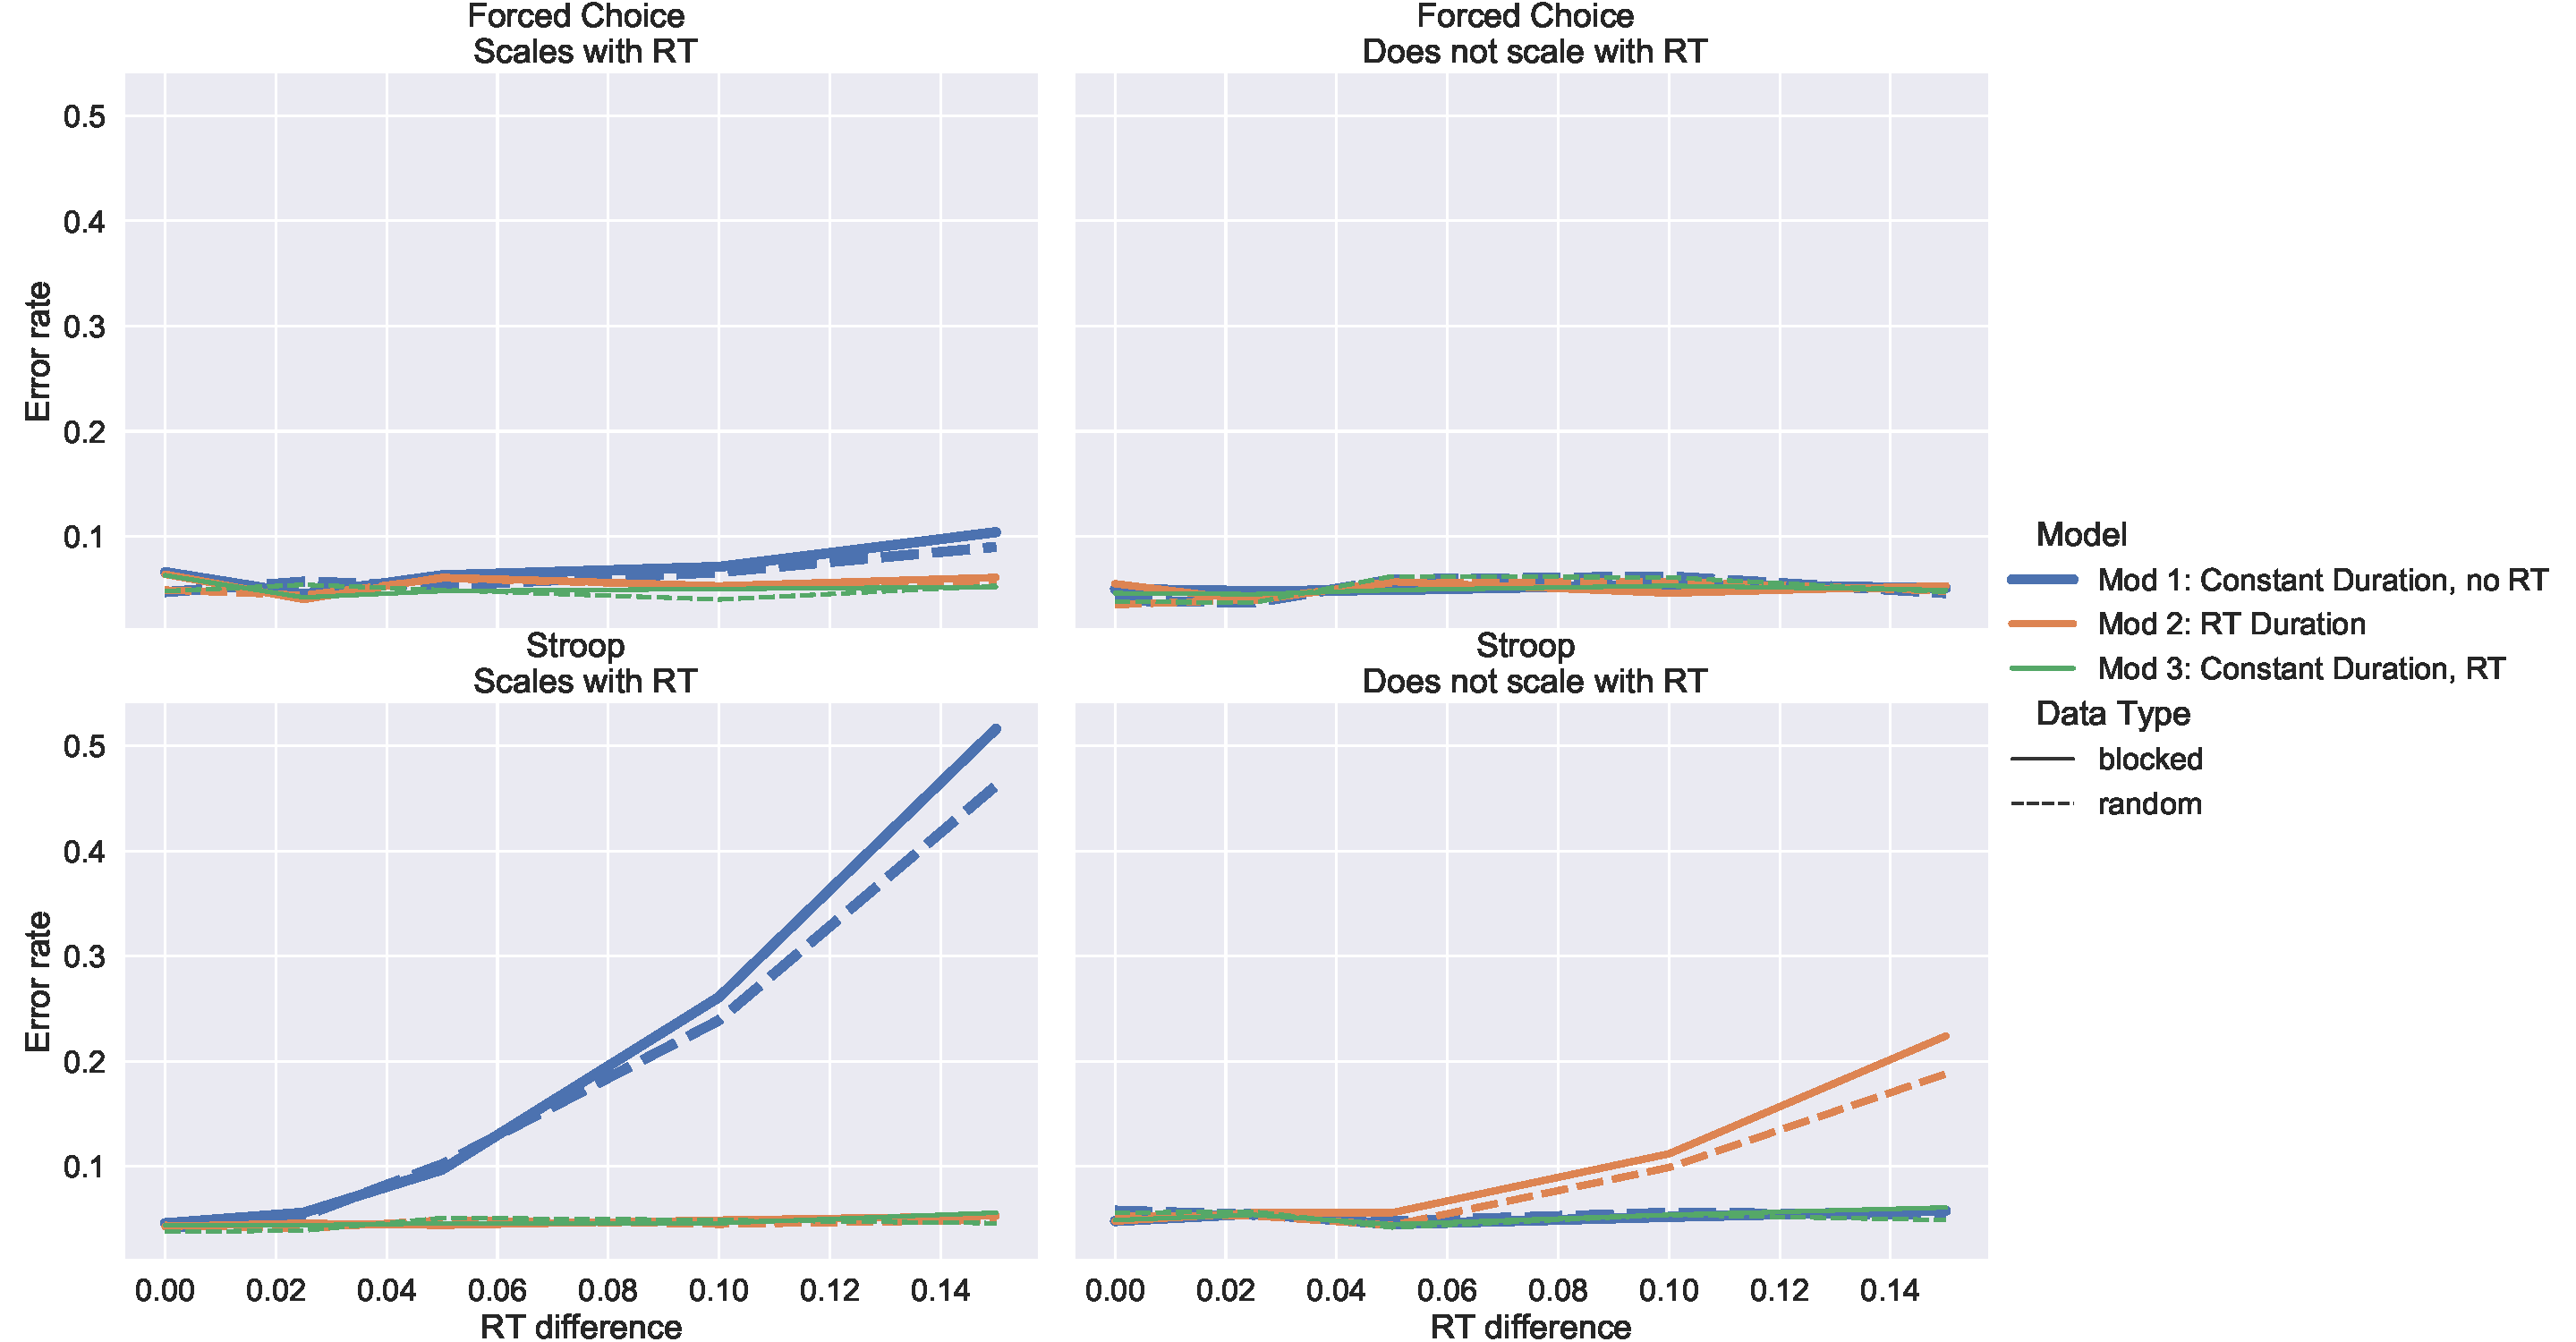
\includegraphics[width=5in]{Figures/type1_err_36.pdf}
   \caption{Type I error as RT difference between conditions increases.  This illustrates that results are similar to when the ISI ranged between 2-4s (result in main manuscript).  The Forced Choice Task RT distribution was used in the top panels, while Stroop RT distribution was used in the bottom panels, both with an ISI between 3-6s was used and inference of interest was the 1-sample t-test of the condition effect with 100 subjects.  2500 simulations were used to calculate the error rate.}
  \label{fig:type1err_36}
\end{figure}




\newpage
\subsection*{Correlation between Stroop effect (incongruent-congruent) with within-subject mean RT differences (incongruent-congruent) when between-trial RT effects are not adjusted for.}
\begin{figure}[h!]
  \centering
   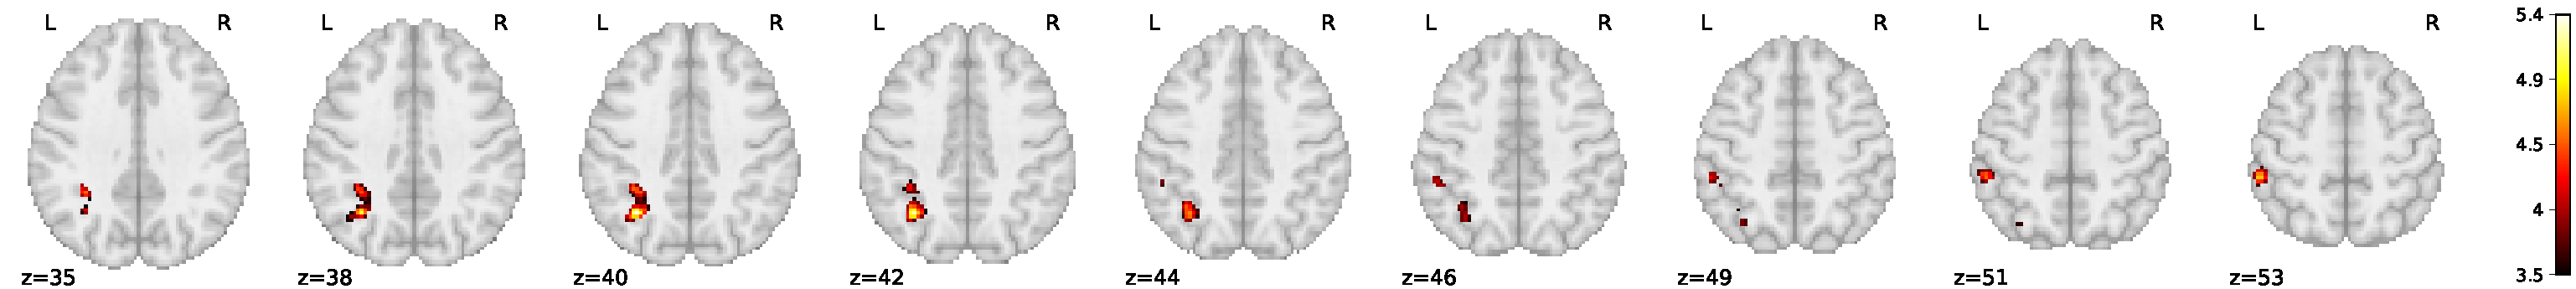
\includegraphics[width=7in]{Figures/stroop_incon_vs_cong_cor_w_rtdiff_nortadj_t_thresh_2sided.pdf}
   \caption{T-statistics for the correlation between the incongruent vs. congruent fMRI contrast and within-subject mean RT differences.  Statistics are thresholded according to a 2-sided p-value$<$0.05, corrected for multiple comparisons using the randomise TFCE statistic (5000 permutations).  Notably there are no significant correlations found if the between-trial RT adjustment is performed using the ConsDurRT model.}
  \label{fig:power}
\end{figure}



\newpage
\subsection*{Average Stroop effect, incongruent vs. congruent, with and without RT adjustment in time series analysis}
\begin{figure}[h!]
  \centering
   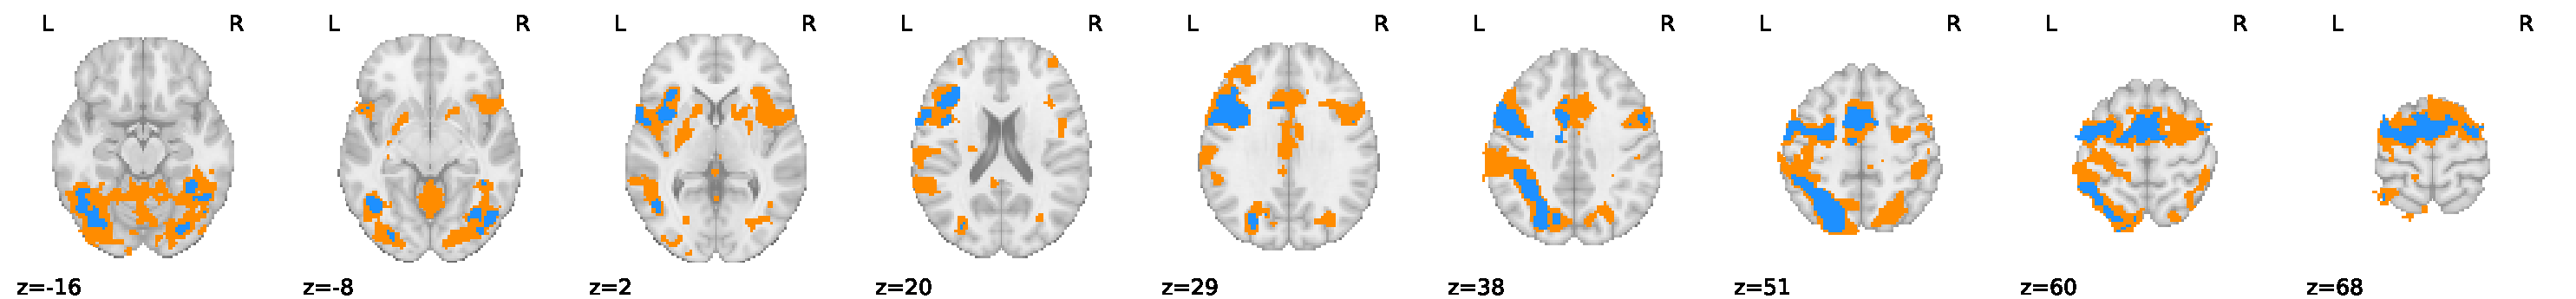
\includegraphics[width=7in]{Figures/stroop_mean_incon_vs_cong_w_rt_blue_wout_rt_orange.pdf}
   \caption{Activation regions for the average Stroop effect (incongruent vs congruent, N=98) with RT adjustment at the time series level (blue) and without (orange).  The group average statistics were thresholded based on randomise TFCE 2-sided t-tests, P$<$0.05. }
  \label{fig: group_corr_stroop}
\end{figure}

\newpage

\subsection*{Details about tasks involved in real data analysis}


The Attention Network Test (ANT) is a task designed to test three attentional networks: (1) alerting, (2) orienting, and (3) executive control. The ANT combines attentional and spatial cues with a flanker task (a central imperative stimulus is flanked by distractors that can indicate the same or opposite response to the imperative stimulus). On each trial a spatial cue is presented, followed by an array of five arrows presented at either the top or the bottom of the computer screen. The subject must indicate the direction of the central arrow in the array of five. The cue that precedes the arrows can be non-existent, a center cue, a double cue (one presented at each of the two possible target locations), or a spatial cue that deterministically indicates the upcoming target location. Each network is assessed via reaction times (RTs). The alerting network contrasts performance with and without cues, the orienting network contrasts performance on the task with or without a reliable spatial cue, and executive control (conflict) is measured by assessing interference from flankers.

The Dot Pattern Expectancy (DPX) task measures individual differences in cognitive control. Participants are presented with a cue made up of dots. This cue can be a valid cue – referred to as A (e.g., ":") – or an invalid cue – referred to as B (e.g., ".."). Next a probe is presented, also made up of a simple dot formation. This probe can be valid (X) or invalid (Y). Participants are instructed to respond to valid probe and cue combinations (targets – AX combinations) with a key press (e.g., “x”) and all others (non-targets) with a different key press (e.g., “m”).

The Kirby Delay-Discounting Task (DDT) is a measure of temporal discounting, the tendency for people to prefer smaller, immediate monetary rewards over larger, delayed rewards. Participants complete a series of 27 questions that each require choosing between a smaller, immediate reward (e.g., \$25 today) versus a larger, later reward (e.g., \$35 in 25 days). The 27 items are divided into three groups according to the size of the larger amount (small, medium, or large). Modeling techniques are used to fit the function that relates time to discounting. The main dependent measure of interest is the steepness of the discounting curve such that a more steeply declining curve represents a tendency to devalue rewards as they become more temporally remote.

The cued task-switching task indexes the control processes involved in reconfiguring the cognitive system to support a new stimulus-response mapping. In this task, subjects are presented with a task cue followed by a colored number (between 1-4 or 6-9). The cue indicates whether to respond based on parity (odd/even), magnitude (greater/less than 5), or color (orange/blue). Trials can present the same cue and task, or can switch the cue or the task. Responses are slower and less accurate when the cue or task differs across trials (i.e. a switch) compared to when the current cue or task remains the same (i.e. a repeat).

The Stop-Signal Task is designed to measure motor response inhibition, one aspect of cognitive control. On each trial of this task participants are instructed to make a speeded response to an imperative ``go'' stimulus except on a subset of trials when an additional ``stop signal'' occurs, in which case participants are instructed that they should make no response. The Independent Race Model describes performance in the Stop-Signal Task as a race between a go process that begins when the go stimulus occurs and a stop process that begins when the stop signal occurs. According to this model, whichever independent process reaches completion first determines the resulting behavior; earlier completion of the go process results in an overt response (i.e., stop-failure), whereas earlier completion of the stop process results in successful inhibition. The main dependent measure, stop-signal reaction time (SSRT), can be computed such that lower SSRT indicates greater response inhibition. One variant of the task measures proactive slowing, the tendency for participants to respond more slowly in anticipation of a potential stopping signal. This variant often uses multiple probabilities of a stop signal (e.g., 20\% and 40\%) to manipulate participants’ expectancies about the likelihood of a stop signal occurring. The extent of slowing in the higher compared to the lower stop probability conditions is an index of proactive slowing/control.

The motor selective stop-signal task measures the ability to engage response inhibition selectively to specific responses. In this task, cues are presented to elicit motor responses (e.g., right hand responses, left hand responses). A stop-signal is presented on some trials, and subjects must stop if certain responses are required on that trial (e.g., right hand responses) but not others (e.g., left hand responses) if a signal occurs. In contrast to a simple stop-signal task in which all actions are stopped when a stop-signal is presented, this task aims to be more like stopping in ``the real world'' in that certain motor actions must be stopped (e.g., stop pressing the accelerator at a red light) but others should proceed (e.g., steering the car and/or conversing with a passenger). Commonly, stop-signal reaction time (SSRT), the main dependent measure for response inhibition in stopping tasks, is prolonged in the motor selective stopping task when compared to the more canonical simple stopping task. This prolongation of SSRT is taken as evidence of the cost of engaging inhibition that is selective to specific effectors or responses.

The Stroop task is a seminal measure of cognitive control. Successful performance of the task requires the ability to overcome automatic tendencies to respond in accordance with current goals. On each trial of the task, a color word (e.g., ``red'', ``blue'') is presented in one of multiple ink colors (e.g., blue, red). Participants are instructed to respond based upon the ink color of the word, not the identity of the word itself. When the color and the word are congruent (e.g., “red” in red ink), the natural tendency to read the word facilitates performance, resulting in fast and accurate responding. When the color and the word are incongruent (e.g., ``red'' in blue ink), the strong, natural tendency to read must be overcome to respond to the ink color. The main dependent measure in the Stroop task is the ``Stroop Effect'', which is the degree of slowing and the reduction in accuracy for incongruent relative to congruent trials.




\end{document}

